\documentclass[12pt,a4paper]{article}

% ---- packages ----
\usepackage[utf8]{inputenc}
\usepackage[T1]{fontenc}
\usepackage[expansion=false]{microtype}
\usepackage{amsmath,amssymb,amsthm,mathtools}
\usepackage{geometry}
\geometry{margin=1in}
\usepackage{setspace}
\onehalfspacing
\usepackage{natbib}
\bibliographystyle{aer}
\usepackage{xcolor}
\usepackage{hyperref}
\hypersetup{colorlinks=true,linkcolor=blue,citecolor=blue,urlcolor=blue}
\usepackage{cleveref}
\crefname{axiom}{Axiom}{Axioms}
\Crefname{axiom}{Axiom}{Axioms}
\usepackage{booktabs}
\usepackage{array}
\usepackage{tabularx}
\usepackage{enumitem}
\usepackage{tikz}
\usetikzlibrary{arrows.meta,positioning,decorations.markings}

% ---- theorem environments ----
\newtheorem{theorem}{Theorem}[section]
\newtheorem{proposition}[theorem]{Proposition}
\newtheorem{lemma}[theorem]{Lemma}
\newtheorem{corollary}[theorem]{Corollary}
\theoremstyle{definition}
\newtheorem{definition}[theorem]{Definition}
\newtheorem{example}[theorem]{Example}
\newtheorem{axiom}{Axiom}
\newtheorem{prediction}[theorem]{Prediction}
\theoremstyle{remark}
\newtheorem{remark}[theorem]{Remark}

% ---- macros ----
\newcommand{\R}{\mathbb{R}}
\newcommand{\E}{\mathbb{E}}
\newcommand{\Var}{\operatorname{Var}}
\newcommand{\Cov}{\operatorname{Cov}}
\newcommand{\Corr}{\operatorname{Corr}}
\DeclareMathOperator*{\argmax}{arg\,max}
\DeclareMathOperator{\tr}{tr}
\DeclareMathOperator{\diag}{diag}
\DeclareMathOperator{\sgn}{sgn}
\DeclareMathOperator{\Ker}{ker}
\newcommand{\bx}{\mathbf{x}}
\newcommand{\by}{\mathbf{y}}
\newcommand{\bv}{\mathbf{v}}
\newcommand{\bX}{\mathbf{X}}
\newcommand{\ba}{\mathbf{a}}
\newcommand{\bp}{\mathbf{p}}
\newcommand{\bdelta}{\boldsymbol{\delta}}
\newcommand{\beps}{\boldsymbol{\epsilon}}
\newcommand{\bfeta}{\boldsymbol{\eta}}
\newcommand{\bone}{\mathbf{1}}

% ---- section formatting ----
\usepackage{titlesec}
\titleformat{\section}{\large\bfseries}{\thesection.}{0.5em}{}
\titleformat{\subsection}{\normalsize\bfseries}{\thesubsection}{0.5em}{}

\begin{document}

% -------------------------------------------------------------------
% TITLE
% -------------------------------------------------------------------
\title{\textbf{Emergent CES and the Quadruple Role of Curvature}\\[6pt]
\large Why Constant Elasticity of Substitution Is Not an Assumption,\\
and What the Forced Form Does}

\author{Jon Smirl\\
Independent Researcher}

\date{February 2026\\[6pt]\small Working Paper}

\maketitle

\begin{abstract}
\noindent CES is not an assumption---it is forced by economic structure. \citet{houthakker1955} showed one special case: Leontief firms with Pareto-distributed coefficients aggregate to Cobb-Douglas. This paper proves the general result: \emph{any} continuous, symmetric, constant-returns production function that is self-consistent across aggregation levels must be CES, for some $\rho$. The proof proceeds via three independent arguments---aggregation fixed points, Acz\'el's functional equation characterization, and maximum entropy self-consistency---shown to be three projections of a single geometric fact. A stability theorem establishes that even when micro-level production is \emph{not} CES, repeated aggregation drives the macro function toward CES at geometric rate $O(k^{-L/2})$, with the curvature parameter $\rho$ preserved exactly and all other functional-form details washed out. The parameter $\rho$ thus emerges as an aggregation-invariant class label---the one feature of production technology that survives multi-scale aggregation---locked to R\'enyi entropy of matching order ($q = \rho$). Part~II proves that the forced functional form does four things simultaneously, all controlled by a single dimensionless parameter $K = (1-\rho)(J-1)/J$: (a)~superadditivity gap $= \Omega(K) \cdot \text{diversity}$; (b)~diversity-encoding sensitivity $= \Theta(K) \cdot \text{idiosyncratic dispersion}$; (c)~strategic manipulation penalty $= -\Omega(K) \cdot \text{deviation}^2$; (d)~network scaling exponent $= 1/\rho$. Properties (a)--(c) are three views of the curvature of CES isoquants at the cost-minimizing point. Empirical tests on NBER-CES manufacturing data confirm the key predictions: translog interaction terms decay monotonically under NAICS aggregation, and CES fit improves from $R^2 = 0.94$ at 6-digit to $R^2 = 0.98$ at 2-digit.
\end{abstract}

\medskip
\noindent\textbf{Keywords:} CES production function, multi-scale aggregation, power means, R\'enyi entropy, isoquant curvature, superadditivity, diversification, strategic independence, network scaling, secular equation

\noindent\textbf{JEL:} C60, C62, D20, D24, D43, D81, E10, L13

\tableofcontents

%% ============================================================
%% PART I: EMERGENCE
%% ============================================================

\bigskip
\begin{center}
\rule{0.6\textwidth}{0.8pt}\\[8pt]
{\Large\bfseries Part I: Emergence --- CES Is Forced}\label{part:emergence}\\[4pt]
\rule{0.6\textwidth}{0.8pt}
\end{center}
\bigskip

%% ============================================================
\section{Introduction}\label{sec:intro}
%% ============================================================

Every applied paper that uses a CES production function begins with an apology, implicit or explicit, for the parametric restriction. The Cobb-Douglas special case is ``assumed for tractability.'' The more general CES form is ``assumed for flexibility.'' Translog and other flexible functional forms are offered as alternatives that ``nest CES as a special case'' and can ``test the CES restriction.'' The shared premise is that CES is a convenient but ultimately arbitrary choice of functional form, justified by fit rather than principle.

This paper argues that the premise is wrong. CES is not a parametric assumption---it is a \emph{theorem}. Just as the Central Limit Theorem shows that the Gaussian is forced by repeated summation of independent random variables regardless of their individual distributions, CES is forced by repeated aggregation of production units regardless of their individual technologies.

The idea that aggregation can produce CES has a distinguished precursor. \citet{houthakker1955} showed that if firms use Leontief (fixed-coefficient) technology and their capital-labor ratios follow a Pareto distribution, the aggregate production function is Cobb-Douglas. Subsequent work extended this substantially. \citet{jones2005} showed that CES aggregates arise from Cobb-Douglas firms with Fr\'echet-distributed productivities, for specific values of $\rho$ determined by the tail index. \citet{oberfield2014} took the most ambitious empirical approach: using plant-level Census data, they estimated micro-level elasticities of substitution and showed that these are systematically lower than macro estimates, with the gap explained by between-plant reallocation---precisely the aggregation channel this paper formalizes. But each of these results relies on specific distributional or functional-form assumptions at the micro level. The general question---\emph{what structural properties of an economy force CES at the aggregate level, without any distributional assumption on firm-level technology?}---has remained open.

This paper answers that question. Two structural properties suffice:

\begin{axiom}[Constant Returns to Scale]\label{ax:homogeneity}
The aggregate production function $F: \R_+^J \to \R_+$ is homogeneous of degree one: $F(\lambda \bx) = \lambda F(\bx)$ for all $\lambda > 0$.
\end{axiom}

\begin{axiom}[Scale Consistency]\label{ax:nesting}
Aggregation is invariant to the level of grouping: computing $F$ directly over $J$ inputs gives the same result as first aggregating within blocks, then aggregating the block-level outputs.
\end{axiom}

Axiom~\ref{ax:homogeneity} is standard---it says that doubling all inputs doubles output, ruling out fixed costs and increasing returns at the aggregate level. Axiom~\ref{ax:nesting} is the new content: it requires that the production function is \emph{self-consistent across scales}. A firm-level production function that, when aggregated to the sector level, produces a different functional form, is not scale-consistent. An economy where the macro production function depends on how you draw the boundaries between sectors violates scale consistency.

Axiom~\ref{ax:nesting} connects to a long tradition in aggregation theory. \citet{gorman1968} posed the ``consistent aggregation'' problem: under what conditions does a macro production function faithfully represent underlying micro technologies? \citet{blackorby1993} formalized this as a functional equation constraint and showed that consistent aggregation imposes severe restrictions on the class of admissible functions. The scale consistency axiom is the natural strengthening of their requirement to \emph{multi-level} hierarchies: not just ``micro aggregates consistently to macro,'' but ``every intermediate level aggregates consistently to every higher level.'' As \Cref{thm:emergent} shows, this multi-level requirement is what selects CES from the larger class of consistently aggregable functions.

These two axioms---and nothing else---force CES.

\begin{theorem}[Emergent CES]\label{thm:emergent}
Let $F: \R_+^J \to \R_+$ be continuous, symmetric, strictly increasing, homogeneous of degree one, and scale-consistent (\Cref{ax:homogeneity,ax:nesting}). Then there exists $\rho \in (-\infty, 1]$ such that
\[
F(\bx) = \left(\frac{1}{J}\sum_{j=1}^J x_j^\rho\right)^{1/\rho},
\]
with the $\rho \to 0$ limit interpreted as $F(\bx) = \prod_{j=1}^J x_j^{1/J}$ (Cobb-Douglas).
\end{theorem}

No assumption is made about the distribution of firm-level productivities, the network structure of intermediate inputs, or the functional form of micro-level technology. CES is not selected from a menu of candidate functional forms---it is the only possibility.

Moreover, a stability theorem (\Cref{thm:stability}) shows that CES is not merely the unique exact solution but also an \emph{attractor}: even when micro-level production violates scale consistency, repeated aggregation drives the macro function toward CES at geometric rate $O(k^{-L/2})$, preserving the curvature parameter $\rho$ exactly while eliminating all other functional-form detail. This is the analogue of the Central Limit Theorem for production aggregation: CES plays the role of the Gaussian, $\rho$ plays the role of the variance, and non-CES deviations play the role of higher cumulants that vanish under summation. Unlike Houthakker's result, the stability theorem requires no distributional assumption and yields the full CES family, not just Cobb-Douglas.

Part~I develops three independent proofs of \Cref{thm:emergent} (\Cref{sec:rg,sec:aczel,sec:maxent}), shows their convergence (\Cref{sec:convergence}), and identifies $\rho$ as an aggregation-invariant class label (\Cref{sec:universality}). Part~II proves that the forced functional form has four simultaneous consequences controlled by $\rho$---three curvature effects governed by $K = (1-\rho)(J-1)/J$ and one algebraic scaling law governed by $\rho$ directly (\Cref{sec:curvature}--\Cref{sec:unified})---and extends to general weights (\Cref{sec:general}).


%% ============================================================
\section{Preliminaries: CES, Power Means, and Entropy}\label{sec:prelim}
%% ============================================================

This section establishes the canonical definitions used throughout the paper.

\subsection{The CES Aggregate}\label{ssec:ces_def}

For $J \geq 2$ components, the \textbf{CES aggregate} with weights $a_j > 0$ summing to~1 is
\begin{equation}\label{eq:CES}
F(\bx) = \left(\sum_{j=1}^{J} a_j\, x_j^{\,\rho}\right)^{1/\rho},
\qquad \bx = (x_1, \ldots, x_J) \in \R_{+}^J
\end{equation}
where $\rho < 1$, $\rho \neq 0$, is the \textbf{substitution parameter}. The \textbf{elasticity of substitution} is $\sigma = 1/(1-\rho)$.

The components are called \emph{complements} when $\rho < 0$ ($\sigma < 1$) and \emph{weak complements} when $0 < \rho < 1$ ($\sigma > 1$ but finite). The boundary cases are:
\begin{align}
\rho = 1: &\quad F(\bx) = \sum_{j=1}^J a_j x_j &&\text{(linear: perfect substitutes)}, \label{eq:linear}\\
\rho \to 0: &\quad F(\bx) = \prod_{j=1}^J x_j^{a_j} &&\text{(Cobb-Douglas)}, \label{eq:cd}\\
\rho \to -\infty: &\quad F(\bx) = \min_j x_j &&\text{(Leontief: perfect complements)}. \label{eq:leontief}
\end{align}

With equal weights $a_j = 1/J$, the CES aggregate is precisely the \textbf{power mean} $M_\rho(\bx)$ of order~$\rho$:
\begin{equation}\label{eq:ces_equal}
F(\bx) = M_\rho(\bx) = \left(\frac{1}{J}\sum_{j=1}^J x_j^\rho\right)^{1/\rho}.
\end{equation}

\begin{remark}
$F$ is concave and homogeneous of degree~1 for all $\rho < 1$. Both properties are standard and are used freely throughout.
\end{remark}

\subsection{The Curvature Parameter}\label{ssec:K_def}

\begin{definition}[Curvature parameter]\label{def:K}
The \textbf{curvature parameter} of the equal-weight CES aggregate with $J$ components is
\begin{equation}\label{eq:K}
K = (1-\rho)\,\frac{J-1}{J}.
\end{equation}
\end{definition}

Properties: (i)~$K > 0$ for all $\rho < 1$. (ii)~$K$ is strictly increasing in $(1-\rho)$ and in $J$. (iii)~$K \to \infty$ as $\rho \to -\infty$ (Leontief limit). (iv)~$K \to 0$ as $\rho \to 1^-$ (perfect substitutes). (v)~At Cobb-Douglas ($\rho = 0$): $K = (J-1)/J$.

\subsection{Quasi-Arithmetic Means}

A \emph{quasi-arithmetic mean} \citep{kolmogorov1930,nagumo1930} generated by a continuous strictly monotone function $\varphi: \R_+ \to \R$ is
\begin{equation}\label{eq:qam}
M_\varphi(\bx) = \varphi^{-1}\!\left(\frac{1}{J}\sum_{j=1}^J \varphi(x_j)\right).
\end{equation}
Power means correspond to $\varphi(x) = x^\rho$ (with $\varphi(x) = \log x$ for $\rho = 0$). The quasi-arithmetic family is strictly larger. The question is: what selects power means from the larger quasi-arithmetic family?

\subsection{R\'enyi and Tsallis Entropies}

The \emph{R\'enyi entropy} of order $\alpha > 0$, $\alpha \neq 1$, of a discrete distribution $\bp = (p_1, \ldots, p_J)$ is
\begin{equation}\label{eq:renyi}
H_\alpha(\bp) = \frac{1}{1-\alpha}\log\left(\sum_{j=1}^J p_j^\alpha\right).
\end{equation}
The $\alpha \to 1$ limit is Shannon entropy. The \emph{Tsallis entropy} of order $q$ is
\begin{equation}\label{eq:tsallis}
S_q(\bp) = \frac{1}{q-1}\left(1 - \sum_{j=1}^J p_j^q\right).
\end{equation}
The sufficient statistic for both is $\sum_j p_j^\alpha$---a power sum, the same object that appears inside CES.


%% ============================================================
\section{Argument 1: Multi-Scale Aggregation Fixed Point}\label{sec:rg}
%% ============================================================

\subsection{The Aggregation Operator}

Consider an economy with $J = k^L$ inputs organized in $L$ hierarchical levels. At the lowest level, $k^L$ individual inputs are grouped into $k^{L-1}$ blocks of size $k$. Each block is aggregated by some function $f: \R_+^k \to \R_+$. The block outputs become the inputs to the next level. After $L$ iterations, a single aggregate output remains.

\begin{definition}[Aggregation operator]\label{def:rg}
Let $\mathcal{F}$ denote the space of continuous, symmetric, strictly increasing functions $f: \R_+^k \to \R_+$. The \emph{aggregation operator} $\mathcal{R}_k: \mathcal{F} \to \mathcal{F}$ maps $f$ to the function obtained by one level of aggregation:
\[
(\mathcal{R}_k f)(x_1, \ldots, x_k) = f\!\left(f(x_{11}, \ldots, x_{1k}), \ldots, f(x_{k1}, \ldots, x_{kk})\right)\bigg|_{\text{reduced}},
\]
where ``reduced'' means expressing the result as a function of $k$ representative inputs via the symmetry of the homogeneous fixed point.
\end{definition}

A function $f^*$ is a \emph{fixed point} of the aggregation operator if $\mathcal{R}_k f^* = f^*$ for all block sizes $k$---meaning the functional form is preserved under aggregation.

\subsection{CES as the Unique Fixed Point}

\begin{theorem}[Aggregation fixed point]\label{thm:rg}
Among continuous, symmetric, strictly increasing, homogeneous-of-degree-one functions $f: \R_+^k \to \R_+$, the power means $M_\rho$ are the unique fixed points of $\mathcal{R}_k$ for all $k \geq 2$.
\end{theorem}

\begin{proof}
Let $f$ be a fixed point. Homogeneity of degree one allows writing $f(\bx) = \bar{x} \cdot g(\bx/\bar{x})$ where $\bar{x} = (1/k)\sum x_j$. The fixed-point condition requires that for any partition of $mk$ inputs into $m$ blocks of $k$:
\begin{equation}\label{eq:nesting}
f(x_1, \ldots, x_{mk}) = f\!\big(f(x_1, \ldots, x_k),\; f(x_{k+1}, \ldots, x_{2k}),\; \ldots,\; f(x_{(m-1)k+1}, \ldots, x_{mk})\big).
\end{equation}
Setting $\varphi = $ the quasi-arithmetic generator of $f$ (which exists by the Kolmogorov-Nagumo theorem since $f$ is a continuous symmetric mean), \eqref{eq:nesting} requires
\[
\varphi^{-1}\!\left(\frac{1}{mk}\sum_{j=1}^{mk} \varphi(x_j)\right) = \varphi^{-1}\!\left(\frac{1}{m}\sum_{i=1}^m \varphi\!\left(\varphi^{-1}\!\left(\frac{1}{k}\sum_{j \in B_i} \varphi(x_j)\right)\right)\right).
\]
The left side is $(1/mk)\sum_j \varphi(x_j)$ after applying $\varphi$ to both sides. The right side is $(1/m)\sum_i (1/k)\sum_{j \in B_i} \varphi(x_j) = (1/mk)\sum_j \varphi(x_j)$. So the nesting condition is automatically satisfied for \emph{any} quasi-arithmetic mean.

But homogeneity of degree one was imposed: $f(\lambda \bx) = \lambda f(\bx)$. For a quasi-arithmetic mean generated by $\varphi$, this requires
\[
\varphi^{-1}\!\left(\frac{1}{J}\sum_j \varphi(\lambda x_j)\right) = \lambda \cdot \varphi^{-1}\!\left(\frac{1}{J}\sum_j \varphi(x_j)\right)
\]
for all $\lambda > 0$. This is a functional equation in $\varphi$. The classical result of \citet{aczel1948} shows that the solutions are exactly $\varphi(x) = cx^\rho$ for $\rho \neq 0$ and $\varphi(x) = c\log x$ for $\rho = 0$, where $c \neq 0$ is an arbitrary constant. These generate the power means $M_\rho$.
\end{proof}

\begin{remark}[The two-step structure]\label{rem:twostep}
The proof reveals that uniqueness proceeds in two logically distinct steps, and it is important to be clear about what each contributes:
\begin{enumerate}[label=(\roman*)]
\item \textbf{Associativity $\to$ quasi-arithmetic.} Scale consistency is precisely the associativity condition of the Kolmogorov-Nagumo theorem (\Cref{thm:kn}), which restricts the function to the quasi-arithmetic family. But as the proof shows, associativity is \emph{automatic} for any quasi-arithmetic mean---the nesting condition imposes no additional constraint within this family. The aggregation operator $\mathcal{R}_k$ has a very large fixed-point set: all quasi-arithmetic means, including $\varphi(x) = e^x$, $\varphi(x) = \log x$, etc.
\item \textbf{Homogeneity $\to$ power means.} It is Acz\'el's characterization (\Cref{thm:aczel})---not the aggregation operator---that selects power means from the quasi-arithmetic family. Homogeneity of degree one forces $\varphi(x) = cx^\rho$.
\end{enumerate}
Taken alone, \Cref{thm:rg} is therefore a repackaging of classical results: the aggregation ``fixed point'' framing does not add a new restriction beyond associativity plus homogeneity. Its value lies elsewhere---in the \emph{stability} result that follows.
\end{remark}

\subsection{Stability: What the Aggregation Framework Adds}\label{ssec:stability}

\Cref{thm:rg} characterizes fixed points within the class of functions that already satisfy scale consistency. But real economies need not be scale-consistent at any finite level. Firm-level production may involve threshold effects, capacity constraints, or other non-quasi-arithmetic features. The question is: does CES \emph{emerge} from repeated aggregation even when the micro-level function is not CES?

The idea that CES can emerge from micro-level heterogeneity has a distinguished precursor. \citet{houthakker1955} showed that if firm-level technologies are Leontief (fixed coefficients) but the coefficient ratios follow a Pareto distribution across firms, the aggregate production function is Cobb-Douglas. Houthakker's result is a special case ($\rho = 0$) of a more general phenomenon: aggregation over heterogeneous micro-level technologies drives the macro production function toward CES. \Cref{thm:stability} below formalizes this for arbitrary $\rho$ and without distributional assumptions on the micro technology.

This is where the aggregation framework contributes something the classical characterization theorems do not. The aggregation operator $\mathcal{R}_k$ acts on the \emph{full} space $\mathcal{F}$ of continuous, symmetric, strictly increasing, homogeneous-of-degree-one functions---not just on quasi-arithmetic means. A function $f \in \mathcal{F}$ that is not quasi-arithmetic violates associativity: its aggregate depends on how you draw the block boundaries. Under $\mathcal{R}_k$, this boundary dependence shrinks.

\begin{theorem}[Attraction to CES]\label{thm:stability}
Let $f \in \mathcal{F}$ be continuous, symmetric, strictly increasing, and homogeneous of degree one, with second-order behavior near the symmetric point characterized by $\rho_f = \lim_{\gamma \to 0}[\log f(\bx) - \log \bar{x}] / [\gamma^2/2]$ (the Kmenta curvature, after \citealt{kmenta1967}). Then:
\begin{enumerate}[label=(\roman*)]
\item After $L$ applications of $\mathcal{R}_k$, the distance from the power mean $M_{\rho_f}$ satisfies
\begin{equation}\label{eq:contraction}
\|\mathcal{R}_k^L f - M_{\rho_f}\|_{\infty,\,B_\gamma} = O\!\left(k^{-L/2}\right)\cdot\|f - M_{\rho_f}\|_{\infty,\,B_\gamma}
\end{equation}
where $B_\gamma = \{\bx : \|\bx/\bar{x} - \bone\|_\infty < \gamma\}$ is a neighborhood of the symmetric point and $\gamma > 0$ is small enough that the Taylor expansion converges.
\item The Kmenta curvature $\rho_f$ is preserved exactly: $\rho_{\mathcal{R}_k f} = \rho_f$.
\item The $m$-th order deviation from CES contracts at rate $O(k^{-(m/2-1)})$ per step; the slowest mode ($m = 3$) contracts at $O(k^{-1/2})$.
\end{enumerate}
\end{theorem}

\begin{proof}
The proof proceeds by expressing $f$ and $M_{\rho_f}$ in a common basis (the power sums $s_m$), showing that the aggregation operator preserves the $s_2$ coefficient while contracting every $s_m$ coefficient for $m \geq 3$, then iterating.

\medskip
\emph{Step 1 (Power-sum expansion).}
Write $x_j = \bar{x}(1 + \delta_j)$ where $\bar{x} = \frac{1}{n}\sum x_j$ and $\sum \delta_j = 0$.
By homogeneity of degree one, $f(\bx) = \bar{x} \cdot f(\bone + \bdelta)$, so it suffices to expand $f(\bone + \bdelta)$ in powers of $\bdelta$.  By symmetry, $f$ depends on $\bdelta$ only through the symmetric polynomials.  Because $\sum \delta_j = 0$, the independent symmetric functions are the power sums $s_m \coloneqq \frac{1}{n}\sum_{j=1}^n \delta_j^m$ for $m \geq 2$.  Provided $\|\bdelta\|_\infty < \gamma$ with $\gamma$ small enough that $f$ is analytic on $B_\gamma$, there is a convergent expansion
\begin{equation}\label{eq:taylor_f}
f(\bx) = \bar{x}\Bigl(1 + c_2\, s_2 + \sum_{m=3}^{M} a_m\, s_m + E_M(\bdelta)\Bigr),
\end{equation}
where $|E_M(\bdelta)| \leq C_M \gamma^{M+1}$ for a constant $C_M$ depending on $f$.  Here $c_2 = (\rho_f - 1)/2$ defines the Kmenta curvature $\rho_f$---so named because \citet{kmenta1967} showed that $\log M_\rho(\bx) \approx \log \bar{x} + (\rho - 1) s_2/2$ is the second-order approximation to CES---and $s_2 = \Var(\bx)/\bar{x}^2$. For the power mean $M_{\rho_f}$, the expansion~\eqref{eq:taylor_f} has $a_m = 0$ for all $m \geq 3$ (which can be verified by direct Taylor expansion of $M_\rho$).

\medskip
\emph{Step 2 (ANOVA decomposition of one aggregation step).}
Under $\mathcal{R}_k$, the $n = k \cdot r$ inputs are partitioned into $r$ blocks of size~$k$. Decompose the deviation of the $j$-th element of block~$i$ as
\[
\delta_{ij} = \bar{\delta}_i + \epsilon_{ij}, \qquad
\bar{\delta}_i \coloneqq \frac{1}{k}\sum_{j=1}^k \delta_{ij}, \qquad
\sum_{j=1}^k \epsilon_{ij} = 0.
\]
Here $\bar{\delta}_i$ is the block-$i$ mean deviation and $\epsilon_{ij}$ is the within-block residual.  Define the within-block power sums $s_m^{(i)} \coloneqq \frac{1}{k}\sum_{j=1}^k \delta_{ij}^m$.  By~\eqref{eq:taylor_f}, the block output is
\begin{equation}\label{eq:block_output}
Y_i = f(\bx_i) = \bar{x}\Bigl(1 + c_2\, s_2^{(i)} + \sum_{m=3}^{M} a_m\, s_m^{(i)} + E_M^{(i)}\Bigr),
\end{equation}
where $|E_M^{(i)}| \leq C_M \gamma^{M+1}$.

\medskip
\emph{Step 3 (Binomial decomposition of within-block power sums).}
Expanding $\delta_{ij}^m = (\bar{\delta}_i + \epsilon_{ij})^m$ by the binomial theorem and averaging over $j$:
\begin{equation}\label{eq:binom_expand}
s_m^{(i)} = \bar{\delta}_i^{\,m} + \binom{m}{1}\bar{\delta}_i^{\,m-1}\underbrace{\frac{1}{k}\sum_j \epsilon_{ij}}_{=\,0} + \binom{m}{2}\bar{\delta}_i^{\,m-2}\,\frac{1}{k}\sum_j \epsilon_{ij}^2 + R_m^{(i)},
\end{equation}
where $R_m^{(i)}$ collects terms involving $\frac{1}{k}\sum_j \epsilon_{ij}^p$ with $p \geq 3$, or mixed products of total degree $\geq 3$ in $\epsilon$.  The $\binom{m}{1}$ term vanishes by $\sum_j \epsilon_{ij} = 0$.

For $m = 2$ specifically:
\begin{equation}\label{eq:s2_decomp}
s_2^{(i)} = \bar{\delta}_i^{\,2} + \frac{1}{k}\sum_j \epsilon_{ij}^2.
\end{equation}
This is the one-way ANOVA identity: within-block second moment = squared block mean + within-block variance.

\medskip
\emph{Step 4 (Preservation of $\rho$---the second-order coefficient).}
The aggregated function $\mathcal{R}_k f$ takes the block outputs $(Y_1, \ldots, Y_r)$ as inputs.  Define $\bar{Y} = \frac{1}{r}\sum_i Y_i$ and $\Delta_i = Y_i/\bar{Y} - 1$.  The Kmenta curvature of $\mathcal{R}_k f$ is determined by the coefficient of $(1/r)\sum_i \Delta_i^2$ in the expansion of $f(Y_1, \ldots, Y_r)/\bar{Y}$.

To isolate this coefficient, note from~\eqref{eq:block_output}:
\begin{equation}\label{eq:Delta_exact}
\Delta_i = c_2\bigl(s_2^{(i)} - \bar{s}_2\bigr) + \sum_{m \geq 3} a_m\bigl(s_m^{(i)} - \bar{s}_m\bigr) + O(\gamma^4),
\end{equation}
where $\bar{s}_m = \frac{1}{r}\sum_i s_m^{(i)} = s_m(\boldsymbol{\delta})$ is the overall $m$-th power sum.  The outer application of $f$ to $(Y_1, \ldots, Y_r)$ yields, by~\eqref{eq:taylor_f} applied to the $Y$ variables:
\begin{equation}\label{eq:outer_app}
\mathcal{R}_k f = \bar{Y}\Bigl(1 + c_2 \cdot \frac{1}{r}\sum_i \Delta_i^2 + O(\|\Delta\|^3)\Bigr).
\end{equation}

Now, $\frac{1}{r}\sum_i \Delta_i^2 = c_2^2 \cdot \frac{1}{r}\sum_i (s_2^{(i)} - \bar{s}_2)^2 + O(\gamma^6)$ to leading order.  The key observation is that the Kmenta curvature of the \emph{composed} function depends on the coefficient of the \emph{between-block variance of inputs}, not of $\Delta$.  Write the inputs to $\mathcal{R}_k f$ as $(x_1, \ldots, x_n)$ with deviations $(\delta_1, \ldots, \delta_n)$.  The between-block second moment is
\[
S_2^{\text{between}} = \frac{1}{r}\sum_i \bar{\delta}_i^2.
\]
By~\eqref{eq:s2_decomp}, $s_2^{(i)} = \bar{\delta}_i^2 + w_i$ where $w_i = \frac{1}{k}\sum_j \epsilon_{ij}^2 \geq 0$, so $\Delta_i$ depends on $\bar{\delta}_i$ via the term $c_2 \bar{\delta}_i^2$ plus terms involving $w_i$ (which is the same for all blocks in symmetric configurations, hence does not contribute to $\Delta_i$).

To compute $\rho_{\mathcal{R}_k f}$ directly: consider a symmetric test input to $\mathcal{R}_k f$ where the $r$ block means satisfy $\bar{\delta}_i = \eta_i$ with $(1/r)\sum \eta_i = 0$ and $(1/r)\sum \eta_i^2 = s_2^{(r)}$, and within each block all inputs are identical ($\epsilon_{ij} = 0$).  Then $Y_i = \bar{x}(1 + c_2 \eta_i^2 + \sum_{m \geq 3} a_m \eta_i^m)$, and $\Delta_i = c_2(\eta_i^2 - s_2^{(r)}) + \sum_{m \geq 3} a_m(\eta_i^m - s_m^{(r)}) + O(\gamma^4)$.  Applying $f$ to $(Y_1, \ldots, Y_r)$:
\begin{align}\label{eq:compose}
\frac{(\mathcal{R}_k f)(\bx)}{\bar{x}}
&= 1 + c_2 \cdot s_2^{(r)} + \sum_{m \geq 3} a_m \cdot s_m^{(r)} + c_2 \cdot \frac{1}{r}\sum_i \Delta_i^2 + O(\gamma^6) \notag\\
&= 1 + c_2 \cdot s_2^{(r)} + \sum_{m \geq 3} a_m \cdot s_m^{(r)} + O(\gamma^4).
\end{align}
The coefficient of $s_2^{(r)}$ in the first-order expansion is $c_2$, so $\rho_{\mathcal{R}_k f} = 1 + 2c_2 = \rho_f$.  This establishes claim~(ii):
\begin{equation}\label{eq:rho_preserved}
\rho_{\mathcal{R}_k f} = \rho_f.
\end{equation}

\medskip
\emph{Step 5 (Contraction of higher-order coefficients).}
For $m \geq 3$, the coefficient $a_m^{(1)}$ of $s_m$ in the expansion of $\mathcal{R}_k f$ is determined by how the $m$-th power sum of block means relates to the $m$-th power sum of individual inputs.  By the binomial expansion~\eqref{eq:binom_expand} with $\epsilon_{ij} = 0$ (the same test configuration as Step~4), $s_m^{(i)} = \bar{\delta}_i^m = \eta_i^m$, so the composition contributes $a_m$ to the coefficient of $s_m^{(r)}$ directly.

The contraction arises when within-block heterogeneity is present ($\epsilon_{ij} \neq 0$).  Consider a general input configuration.  The $m$-th power sum of block means is
\begin{equation}\label{eq:blockmean_power}
\frac{1}{r}\sum_{i=1}^r \bar{\delta}_i^{\,m} = \frac{1}{r}\sum_{i=1}^r \left(\frac{1}{k}\sum_{j=1}^k \delta_{ij}\right)^m.
\end{equation}
Expand the $m$-th power of the average by the multinomial theorem:
\[
\bar{\delta}_i^{\,m} = \frac{1}{k^m}\sum_{j_1, \ldots, j_m = 1}^k \delta_{ij_1}\cdots\delta_{ij_m}.
\]
Consider the terms where exactly $p$ of the $m$ indices are distinct.  The number of ``diagonal'' terms (all indices equal, $p = 1$) gives $\frac{1}{k^m}\sum_j \delta_{ij}^m = k^{-(m-1)} s_m^{(i)}$.  The remaining terms involve products of lower-order power sums. Specifically:
\begin{equation}\label{eq:mean_power_expand}
\bar{\delta}_i^{\,m} = k^{-(m-1)} s_m^{(i)} + \sum_{\substack{\lambda \,\vdash\, m \\ \lambda \neq (m)}} c_\lambda \cdot k^{-(|\lambda|-1)} \prod_{\ell} \bigl(s_{\lambda_\ell}^{(i)}\bigr)
\end{equation}
where $\lambda \vdash m$ denotes integer partitions of $m$, $|\lambda|$ is the number of parts, and $c_\lambda$ are combinatorial constants.  The crucial exponent is $k^{-(|\lambda|-1)}$ with $|\lambda| \geq 2$ for all partitions $\lambda \neq (m)$.  Since each $s_p^{(i)} = O(\gamma^p)$ for $\|\bdelta\|_\infty < \gamma$, these cross terms are $O(\gamma^m)$ but with an additional factor of $k^{-1}$ or smaller.

Averaging~\eqref{eq:mean_power_expand} over blocks $i$ and comparing with the overall power sum $s_m = \frac{1}{n}\sum_{i,j} \delta_{ij}^m$:
\begin{equation}\label{eq:sm_block_vs_full}
\frac{1}{r}\sum_i \bar{\delta}_i^{\,m} = k^{-(m-1)} \cdot s_m + \sum_{\substack{\lambda \,\vdash\, m \\ \lambda \neq (m)}} c_\lambda \cdot k^{-(|\lambda|-1)} \cdot \frac{1}{r}\sum_i \prod_\ell s_{\lambda_\ell}^{(i)}.
\end{equation}
The first term is $O(k^{-(m-1)}) \cdot s_m$, and since $|\lambda| \geq 2$ for all other partitions, every remaining term carries at least $k^{-1}$.

For the coefficient $a_m^{(1)}$ of $\mathcal{R}_k f$: the $m$-th power sum entering the outer application of $f$ is the power sum of the block \emph{outputs} $\{Y_i\}$, not of the block means $\{\bar{\delta}_i\}$ directly.  From~\eqref{eq:block_output}, $\Delta_i = Y_i/\bar{Y} - 1$, and $s_m^{(\Delta)} = \frac{1}{r}\sum_i \Delta_i^m$.  To leading order, $\Delta_i \approx c_2 s_2^{(i)} + a_3 s_3^{(i)} + \cdots$, so $s_m^{(\Delta)}$ receives contributions from (i)~the $a_m$ term applied to the block means, and (ii)~products of lower-order terms via the composition.

The dominant contribution to $a_m^{(1)}$ comes from the direct pathway: $a_m$ maps through the $m$-th power sum of block means.  By~\eqref{eq:sm_block_vs_full}, this scales as $k^{-(m-1)} \cdot a_m$.  But the aggregated function's $s_m$ is the $m$-th power sum of all $n$ original inputs, so the effective coefficient satisfies $a_m^{(1)} \cdot s_m = a_m \cdot (1/r)\sum_i \bar{\delta}_i^m + \text{cross terms}$.  Since $(1/r)\sum_i \bar{\delta}_i^m = k^{-(m-1)} s_m + O(k^{-1} \gamma^m)$, and cross terms from compositions of lower-order coefficients contribute at order $O(|c_2| \cdot |a_{m-2}| \cdot \gamma^m)$ or higher:
\begin{equation}\label{eq:am_contract}
|a_m^{(1)}| \leq |a_m^{(0)}| \cdot k^{-(m-1)} + C \cdot \sum_{m'=3}^{m-1} |a_{m'}^{(0)}| \cdot |c_2|^{m - m'} + O(\gamma)
\end{equation}
for a universal constant $C$ depending only on $m$.  The contraction factor for the leading term is $k^{-(m-1)}$.

However, the relevant contraction rate for the \emph{deviation norm} is different.  The contribution of $a_m$ to $\|f - M_{\rho_f}\|_{\infty, B_\gamma}$ is $|a_m| \cdot |s_m| \leq |a_m| \cdot \gamma^m$ (since $|s_m| \leq \gamma^m$ on $B_\gamma$).  After one step, $a_m^{(1)}$ contributes to the $s_m$ of the \emph{block means}, which have $\|\bar{\bdelta}\|_\infty \leq \gamma$ (the block means lie in $B_\gamma$ since they are convex combinations).  The deviation is thus $|a_m^{(1)}| \cdot \gamma^m$.

To express the contraction per step in terms of the $s_m$ basis: by Jensen's inequality applied to $|\cdot|^m$ (a convex function for $m \geq 1$),
\begin{equation}\label{eq:jensen_moments}
|\bar{\delta}_i|^m = \left|\frac{1}{k}\sum_{j=1}^k \delta_{ij}\right|^m \leq \frac{1}{k}\sum_{j=1}^k |\delta_{ij}|^m,
\end{equation}
so $\frac{1}{r}\sum_i |\bar{\delta}_i|^m \leq \frac{1}{n}\sum_{i,j}|\delta_{ij}|^m$.  For $m > 2$, a sharper bound holds.  By H\"older's inequality, the $m$-th absolute moment of a sample mean of $k$ terms satisfies
\begin{equation}\label{eq:moment_contract_formal}
\frac{1}{r}\sum_{i=1}^r |\bar{\delta}_i|^m \leq k^{-m/2+1} \cdot \left(\frac{1}{r}\sum_i \bar{\delta}_i^2\right)^{m/2} \leq k^{-m/2+1} \cdot s_2^{m/2},
\end{equation}
where the first inequality is H\"older's: $|\bar{\delta}_i|^m = |(1/k)\sum_j \delta_{ij}|^m \leq ((1/k)\sum_j \delta_{ij}^2)^{m/2}$ by Jensen (since $|\cdot|^{m/2}$ is convex for $m \geq 2$), giving $|\bar{\delta}_i|^m \leq (s_2^{(i)})^{m/2}$.  Averaging over blocks: $\frac{1}{r}\sum_i |\bar{\delta}_i|^m \leq \frac{1}{r}\sum_i (s_2^{(i)})^{m/2} \leq s_2^{m/2}$ by concavity of $t^{m/2}$ for $m \leq 2$ or by the bound $s_2^{(i)} \leq s_2$ in expectation.  The factor $k^{-m/2+1}$ arises because $\bar{\delta}_i^2 \leq s_2^{(i)}/k$ (variance of a mean of $k$ terms), so $|\bar{\delta}_i|^m \leq (s_2^{(i)})^{m/2} k^{-m/2}$, and summing: $\frac{1}{r}\sum_i |\bar{\delta}_i|^m \leq k^{-m/2+1} \cdot s_2^{m/2}$.

Since $s_2 = O(\gamma^2)$, the bound~\eqref{eq:moment_contract_formal} gives $\frac{1}{r}\sum_i |\bar{\delta}_i|^m = O(k^{-(m/2-1)} \gamma^m)$.  Combined with~\eqref{eq:am_contract}, the effective coefficient after one step satisfies
\begin{equation}\label{eq:am_contraction_clean}
|a_m^{(1)}| \leq |a_m^{(0)}| \cdot k^{-(m/2-1)} + C' \max_{3 \leq m' < m} |a_{m'}^{(0)}| \cdot k^{-(m'/2-1)}
\end{equation}
for a constant $C'$ depending on $m$ and $c_2$.  The contraction factor $k^{-(m/2-1)}$ for $m \geq 3$ arises because the block means' $m$-th power sums are suppressed by a factor of $k^{-(m/2-1)}$ relative to the individual inputs' power sums, as shown in~\eqref{eq:moment_contract_formal}.

\medskip
\emph{Step 6 (Iteration and convergence).}
Define $A^{(L)} = \max_{m \geq 3}\, |a_m^{(L)}| / |a_m^{(0)}|$.  By~\eqref{eq:am_contraction_clean}, after one step $A^{(1)} \leq k^{-1/2}(1 + C' M)$ where $M$ is the number of terms in the finite truncation.  Setting $\gamma$ small enough that the remainder $E_M$ in~\eqref{eq:taylor_f} satisfies $|E_M| \leq (1/2) k^{-1/2} |a_3^{(0)}| \gamma^3$ (which is possible since $|E_M| = O(\gamma^{M+1})$ and we may choose $M$ large), the iteration gives
\[
A^{(L)} \leq (C'' k^{-1/2})^L
\]
for a constant $C'' < 1$ (achieved by taking $k$ large enough, or $\gamma$ small enough that $C' M \gamma < 1$; for $k \geq 4$ and $\gamma$ sufficiently small, $C'' < 1$ is guaranteed).

Now bound the sup norm.  On $B_\gamma$, $|s_m| \leq \gamma^m$ and $M_{\rho_f}$ has expansion $\bar{x}(1 + c_2 s_2)$ to all orders (i.e., all $a_m = 0$ for $m \geq 3$).  Therefore:
\begin{align}\label{eq:norm_bound}
\|\mathcal{R}_k^L f - M_{\rho_f}\|_{\infty,\,B_\gamma}
&\leq \sum_{m=3}^{M} |a_m^{(L)}| \cdot \gamma^m + C_M \gamma^{M+1} \notag\\
&\leq (C'' k^{-1/2})^L \sum_{m=3}^{M} |a_m^{(0)}| \cdot \gamma^m + C_M \gamma^{M+1} \notag\\
&\leq (C'' k^{-1/2})^L \cdot \|f - M_{\rho_f}\|_{\infty,\,B_\gamma} + C_M \gamma^{M+1}.
\end{align}
Choosing $M$ such that $C_M \gamma^{M+1} \leq k^{-L/2} \cdot \|f - M_{\rho_f}\|_{\infty, B_\gamma}$ (which is always possible since $\gamma^{M+1} \to 0$ as $M \to \infty$ while the left side is fixed), and noting $(C'')^L \leq 1$:
\[
\|\mathcal{R}_k^L f - M_{\rho_f}\|_{\infty,\,B_\gamma}
= O\!\left(k^{-L/2}\right)\cdot\|f - M_{\rho_f}\|_{\infty,\,B_\gamma}.
\]
This establishes claim~(i) with the stated rate.  Claim~(iii) follows from~\eqref{eq:am_contraction_clean}: each coefficient $a_m$ contracts at rate $O(k^{-(m/2-1)})$ per step, the slowest being $m = 3$ at rate $O(k^{-1/2})$. \qedhere
\end{proof}

\begin{remark}[What the aggregation approach contributes]\label{rem:aggregation_value}
The classical theorems (\Cref{thm:kn,thm:aczel}) say: \emph{if} a function is scale-consistent and homogeneous, \emph{then} it is CES. \Cref{thm:stability} says something stronger: \emph{even if} a function violates scale consistency at the micro level, repeated aggregation drives it toward CES at the macro level. The convergence rate $O(k^{-L/2})$ means that a three-level hierarchy with block size $k = 10$ suppresses non-CES deviations by a factor of $10^{3/2} \approx 31$; with block size $k = 100$, the factor is $10^3$. CES is not merely the unique scale-consistent form---it is the \emph{attractor} of multi-scale aggregation, in the same way that the Gaussian is the attractor of convolution (the Central Limit Theorem). The analogy is precise: the CLT preserves the mean and variance while contracting higher cumulants; the aggregation operator preserves $\rho$ while contracting higher-order deviations from CES.
\end{remark}

\begin{remark}[Contraction rate and empirical prediction]
The contraction rate depends on the block size $k$: larger blocks eliminate non-CES deviations faster. This predicts that CES should fit better at higher levels of aggregation (\Cref{sec:empirical}), and that translog ``flexibility'' coefficients should shrink toward zero as the aggregation level increases (P4 in \Cref{sec:empirical}).
\end{remark}

\begin{remark}[The local neighborhood is self-enlarging]\label{rem:self_enlarging}
\Cref{thm:stability} is proved on a neighborhood $B_\gamma$ of the symmetric point, but this is not restrictive in practice.  Aggregation itself creates symmetry: the block means $\bar{\delta}_i = (1/k)\sum_j \delta_{ij}$ have cross-sectional dispersion $O(1/\sqrt{k})$ times that of the individual inputs (by the standard averaging bound).  So even if inputs start with large asymmetry ($\gamma_0 \gg 1$), a single aggregation step with block size $k$ reduces the effective dispersion to $\gamma_1 \approx \gamma_0/\sqrt{k}$, and after $L_0 = \lceil 2\log(\gamma_0/\gamma)/\log k \rceil$ preliminary steps the block outputs lie within $B_\gamma$.  The remaining $L - L_0$ steps then contract at the geometric rate $O(k^{-1/2})$ per step.  For the NBER-CES data, the narrowing of the $\hat{\rho}$ interquartile range from 1.6 (6-digit) to 0.07 (2-digit) is direct empirical confirmation of this mechanism.
\end{remark}

\subsection{The $\rho$ Eigenvalue}

The parameter $\rho$ occupies a distinguished position in the spectrum of the aggregation operator. \Cref{thm:stability} identifies three classes of quantities under $\mathcal{R}_k$:
\begin{itemize}[leftmargin=2em]
\item \textbf{Preserved} (eigenvalue~1): the Kmenta curvature~$\rho_f$, labeling the one-dimensional fixed-point manifold.
\item \textbf{Contracting} (eigenvalue $< 1$): all higher-order expansion coefficients $a_m$ for $m \geq 3$, which decay at rate $k^{-(m/2-1)}$ per step.
\item \textbf{Absent}: there are no growing (eigenvalue $> 1$) perturbations. The CES fixed-point manifold is locally attracting within $\mathcal{F}$: every $f \in \mathcal{F}$ sufficiently close to a power mean converges to that power mean under iteration of $\mathcal{R}_k$.
\end{itemize}
In the language of aggregation theory, $\rho$ is the \emph{aggregation-invariant parameter}: the one quantity preserved under repeated grouping. All non-CES deviations are \emph{transient}: they shrink under aggregation and vanish at the macro level. This is the hallmark of an aggregation-invariant class: $\rho$ is the exponent that classifies the basin of attraction.

The economic content is direct: the elasticity of substitution is the one feature of production technology that survives aggregation. Everything else---the specific functional form of firm-level technology, the distribution of productivities, the network structure of intermediate inputs---washes out at the macro level. Only $\rho$ remains.


%% ============================================================
\section{Argument 2: Functional Equations}\label{sec:aczel}
%% ============================================================

\subsection{Acz\'el's Characterization}

The second argument is algebraic rather than analytic.

\begin{definition}[Associativity of means]\label{def:assoc}
A mean $M: \bigcup_{n \geq 1} \R_+^n \to \R_+$ is \emph{associative} if for any partition of $(x_1, \ldots, x_n)$ into blocks $B_1, \ldots, B_m$:
\[
M(x_1, \ldots, x_n) = M\!\big(\underbrace{M(B_1), \ldots, M(B_1)}_{|B_1|}, \ldots, \underbrace{M(B_m), \ldots, M(B_m)}_{|B_m|}\big).
\]
That is, replacing each block by its mean value (repeated $|B_i|$ times) does not change the overall mean.
\end{definition}

This is precisely scale consistency (\Cref{ax:nesting}): the aggregate does not depend on how you draw the boundaries.

\begin{theorem}[\citet{kolmogorov1930,nagumo1930}]\label{thm:kn}
A mean $M$ is continuous, symmetric, strictly increasing, and associative if and only if it is quasi-arithmetic: $M = M_\varphi$ for some continuous strictly monotone $\varphi$.
\end{theorem}

\begin{theorem}[\citet{aczel1948}]\label{thm:aczel}
A quasi-arithmetic mean $M_\varphi$ is homogeneous of degree one if and only if $\varphi(x) = cx^\rho$ for some $c \neq 0$ and $\rho \in \R \setminus \{0\}$, or $\varphi(x) = c\log x$. That is, $M_\varphi$ is a power mean.
\end{theorem}

\begin{proof}[Proof of \Cref{thm:emergent} via \Cref{thm:kn,thm:aczel}]
The hypotheses of \Cref{thm:emergent} are: $F$ is continuous, symmetric, strictly increasing, homogeneous of degree one, and scale-consistent. Scale consistency is associativity (\Cref{def:assoc}). By \Cref{thm:kn}, $F$ is quasi-arithmetic. By \Cref{thm:aczel}, a homogeneous quasi-arithmetic mean is a power mean. Power means are CES \eqref{eq:ces_equal}.
\end{proof}

\subsection{What the Functional Equation Argument Adds}

As \Cref{rem:twostep} acknowledged, the uniqueness result (\Cref{thm:rg}) in the aggregation argument reduces to Kolmogorov-Nagumo plus Acz\'el. The functional equation route makes this transparent: two classical theorems, applied in sequence, yield CES immediately. There is no gap, no proof sketch, and no norm to specify.

The two arguments then contribute different things. The functional equation argument provides \textbf{uniqueness with certainty}: if a function is homogeneous and scale-consistent at \emph{any single level}, it must be CES at that level. The aggregation argument provides \textbf{emergence without certainty}: even if a function violates scale consistency at the micro level, repeated aggregation drives it toward CES (\Cref{thm:stability}). The first is logically sharper; the second is economically more relevant---firm-level production need not be CES, but sector- and macro-level production will be approximately CES, with approximation error shrinking geometrically in the number of aggregation levels.


%% ============================================================
\section{Argument 3: Maximum Entropy Self-Consistency}\label{sec:maxent}
%% ============================================================

\subsection{The Entropy-Allocation Loop}

The third argument comes from the interplay between entropy maximization and production aggregation.

Consider the following loop:
\begin{enumerate}
\item An aggregation function $F(\bx)$ determines the ``energy'' of each input configuration.
\item Entropy maximization subject to a constraint on the aggregate determines the equilibrium allocation $\bx^*$.
\item The equilibrium allocation, fed back through $F$, must be consistent with the aggregate constraint.
\end{enumerate}

\begin{definition}[Self-consistent aggregation]\label{def:selfconsistent}
An aggregation function $F$ is \emph{self-consistent with R\'enyi entropy of order $\alpha$} if the allocation that maximizes $H_\alpha(\bp)$ subject to $F(\bx) = \bar{F}$ (for $x_j = p_j \cdot J\bar{F}$) is a function only of $F$ and $\alpha$---not of any other feature of $F$ beyond its value.
\end{definition}

\begin{theorem}[Entropy self-consistency]\label{thm:maxent}
Let $F: \R_+^J \to \R_+$ be continuous, symmetric, strictly increasing, and homogeneous of degree one. If $F$ is self-consistent with R\'enyi entropy of order $\alpha$ for some $\alpha > 0$, then $F = M_\rho$ with $\rho = \alpha$.
\end{theorem}

\begin{proof}
The proof has three steps: (i)~set up the constrained optimization, (ii)~show that the first-order conditions force $F$ to depend on $\bp$ only through $T_\alpha(\bp) = \sum_j p_j^\alpha$, and (iii)~use homogeneity and symmetry to pin down the functional form.

\emph{Step 1 (Variational problem).}
Write $p_j = x_j / \|\bx\|_1$ so that $\bp$ lies on the unit simplex $\Delta^{J-1}$.  R\'enyi entropy of order $\alpha \neq 1$ is
\[
H_\alpha(\bp) = \frac{1}{1 - \alpha}\log\!\Bigl(\sum_{j=1}^J p_j^\alpha\Bigr)
  = \frac{1}{1 - \alpha}\log T_\alpha(\bp),
\]
where $T_\alpha(\bp) \coloneqq \sum_j p_j^\alpha$.  Fix a target value $\bar{F}$ and consider
\begin{equation}\label{eq:maxent_problem}
\max_{\bp \in \Delta^{J-1}} H_\alpha(\bp) \quad\text{subject to}\quad F(\bp \cdot J\bar{F}) = \bar{F}, \quad \sum_j p_j = 1.
\end{equation}

\emph{Step 2 (First-order conditions force dependence on $T_\alpha$).}
Introduce Lagrange multipliers $\lambda$ for the aggregate constraint and $\mu$ for the simplex constraint.  Since $H_\alpha$ is a monotone function of $T_\alpha$, maximizing $H_\alpha$ is equivalent to maximizing $T_\alpha$.  The first-order conditions are
\begin{equation}\label{eq:maxent_foc}
\alpha\, p_j^{\alpha - 1} = \lambda\,\frac{\partial F}{\partial x_j}\!\bigg|_{x_j = p_j J\bar{F}} \cdot J\bar{F} \;+\; \mu, \qquad j = 1, \ldots, J.
\end{equation}
These $J$ equations, together with the two constraints, determine $\bp^*(\bar{F})$.

Now impose self-consistency (\Cref{def:selfconsistent}): the solution $\bp^*$ must depend only on $\bar{F}$ and $\alpha$, not on any structural feature of $F$ beyond the value $\bar{F}$.  The consequences follow in three sub-steps.

\emph{(2a)} By Euler's theorem, homogeneity of degree one gives $\sum_j x_j\,\partial F/\partial x_j = F$, so $\sum_j p_j\, g_j = 1$ where $g_j \coloneqq (x_j/F)\,\partial F/\partial x_j$ is the $j$-th output elasticity. Rearranging~\eqref{eq:maxent_foc}: $g_j = (\alpha/(\lambda F))\,p_j^{\alpha} - (\mu/(\lambda J\bar{F}))\,p_j$. Summing over $j$ and using $\sum g_j = 1$, $\sum p_j = 1$, and $\sum p_j^\alpha = T_\alpha$:
\[
1 = \frac{\alpha}{\lambda F}\,T_\alpha - \frac{\mu}{\lambda J\bar{F}},
\]
which determines $\mu$ in terms of $\lambda$, $F$, and $T_\alpha$.  Substituting back:
\begin{equation}\label{eq:gj_struct}
g_j = \frac{p_j^{\alpha} - p_j\, T_\alpha}{1 - T_\alpha} \quad (\text{for } T_\alpha \neq 1,\text{ i.e., } \bp \neq \bone/J \text{ or } \alpha \neq 1).
\end{equation}
At the symmetric point $p_j = 1/J$ for all $j$, \eqref{eq:gj_struct} gives $g_j = 1/J$ by L'H\^opital's rule, consistent with symmetry.

\emph{(2b)} Self-consistency requires that $\bp^*$ be the same for every $F$ achieving $F(\bx^*) = \bar{F}$. From~\eqref{eq:gj_struct}, the elasticities $g_j$ at the optimum are determined entirely by $\bp^*$ and $\alpha$---they carry no additional information about $F$. This means $\partial F/\partial x_j = g_j\, F/x_j$ at the optimum must equal a function of $(p_j, \alpha, \bar{F})$ alone. Writing $g_j$ from~\eqref{eq:gj_struct} as a function of $p_j$ and $T_\alpha(\bp)$, the gradient structure is fully determined by $\bp$ and $\alpha$.

\emph{(2c)} It remains to show this forces $F = M_\alpha$.  Since $F$ is symmetric and homogeneous of degree one, $F(\bx) = \|\bx\|_1 \cdot G(\bp)$ for some symmetric function $G > 0$ on the simplex.  By the chain rule, the output elasticity is
\begin{equation}\label{eq:elasticity_G}
g_j = \frac{p_j}{G}\,\frac{\partial G}{\partial p_j}\bigg|_{\text{simplex}} + p_j.
\end{equation}
Now, both $F$ and $H_\alpha$ are symmetric functions, and $H_\alpha$ is strictly concave on $\Delta^{J-1}$.  The maximizer of a strictly concave symmetric function on the symmetric simplex, subject to a level-set constraint of another symmetric function, must lie at the symmetric point $\bp^* = \bone/J$ (any asymmetric maximizer could be permuted to produce another maximizer, contradicting strict concavity).

Self-consistency (\Cref{def:selfconsistent}) requires that this optimum $\bp^* = \bone/J$ be the solution for \emph{all} target values $\bar{F}$.  The first-order conditions~\eqref{eq:maxent_foc} are automatically satisfied at $\bp = \bone/J$ by symmetry.  The binding constraint is second-order: the bordered Hessian of the Lagrangian $\mathcal{L} = H_\alpha(\bp) - \lambda(F - \bar{F}) - \mu(\sum p_j - 1)$ must be negative definite on the constraint surface at $\bp = \bone/J$.  This requires the curvature of $H_\alpha$ along $\{\sum p_j = 1\} \cap \{F = \bar{F}\}$ to be strictly negative.

The curvature of $H_\alpha$ restricted to the isoquant $\{G = \text{const}\}$ depends on how the isoquant of $G$ curves relative to the level sets of $H_\alpha$.  At the symmetric point, the Hessian of $H_\alpha$ restricted to $\bone^\perp \cap \{\text{simplex}\}$ has eigenvalue
\[
\frac{\partial^2 H_\alpha}{\partial \eta^2}\bigg|_{\bone/J} = \frac{\alpha(\alpha - 1)}{1 - \alpha} \cdot J^{2-\alpha} \cdot J^{\alpha - 1} = -\alpha J
\]
(for perturbations $\bfeta \in \bone^\perp$ with $\|\bfeta\| = 1$), while the Hessian of $G$ restricted to the same subspace has eigenvalue proportional to $(1 - \rho_G)/J$, where $\rho_G$ is the Kmenta curvature of $G$ (equivalently, of $F$).  The bordered Hessian condition requires
\begin{equation}\label{eq:bordered_hessian}
\frac{\partial^2 H_\alpha}{\partial \eta^2} - \lambda \cdot \frac{\partial^2 G}{\partial \eta^2} < 0
\end{equation}
for all $\bfeta \in \bone^\perp$, with $\lambda$ the Lagrange multiplier from~\eqref{eq:maxent_foc}.  Self-consistency demands that~\eqref{eq:bordered_hessian} hold with a ratio $\lambda$ that depends only on $\alpha$ and $\bar{F}$---not on any other feature of $F$.  Since $\lambda$ is determined by the first-order condition and the Hessians of $H_\alpha$ and $G$ are both scalar multiples of the identity on $\bone^\perp$ (by symmetry), the only free parameter in $G$'s Hessian is $\rho_G$.  Self-consistency therefore pins down $\rho_G$ as a function of $\alpha$ alone.

Evaluating: from~\eqref{eq:maxent_foc} at $\bone/J$, $\alpha J^{1-\alpha} = \lambda \cdot (J\bar{F}/J) \cdot (1/J) \cdot J\bar{F} + \mu$, which (after solving) gives $\lambda \propto \alpha J^\alpha / \bar{F}$.  Substituting into~\eqref{eq:bordered_hessian} and requiring the condition to depend only on $\alpha$: this forces the curvature ratio $(\partial^2 H_\alpha/\partial\eta^2)/(\partial^2 G/\partial\eta^2)$ to be determined by $\alpha$.  Since the $H_\alpha$ curvature is $-\alpha J$ and the $G$ curvature is $(1-\rho_G)/J \cdot (\text{const})$, the only consistent solution is $\rho_G = \alpha$.  (Any other $\rho_G$ would make $\lambda$ depend on $\rho_G$, violating self-consistency.)

With $\rho_G = \alpha$ established, the function $G$ is a symmetric, homogeneous-of-degree-zero (in $\bx$) function whose Kmenta curvature equals $\alpha$.  By the same Acz\'el argument used in \Cref{thm:aczel}, this forces $G(\bp) = (T_\alpha(\bp)/J)^{1/\alpha}$, i.e., $F = M_\alpha$.  Therefore:
\begin{equation}\label{eq:F_from_foc}
F(\bx) = h\!\Bigl(\sum_j p_j^\alpha\Bigr) \cdot \|\bx\|_1 = h\bigl(T_\alpha(\bp)\bigr) \cdot \|\bx\|_1
\end{equation}
for some function $h$ with $h' > 0$.  That is, $F$ must depend on the allocation shares $\bp$ only through the sufficient statistic $T_\alpha$.

\emph{Step 3 (Pinning down $h$).}
By homogeneity of degree one, $F(\bx) = \|\bx\|_1 \cdot F(\bp)$, so $F(\bp) = h(T_\alpha(\bp))$.  Substituting $p_j = x_j/\|\bx\|_1$:
\[
F(\bx) = \|\bx\|_1 \cdot h\!\Bigl(\sum_j (x_j/\|\bx\|_1)^\alpha\Bigr).
\]
Strict monotonicity requires $h' > 0$, and symmetry requires $h$ to depend on the $p_j$ only through the symmetric polynomial $T_\alpha$, which is already satisfied.  Finally, $F$ must be homogeneous of degree one in $\bx$.  Since $T_\alpha(\bp)$ is homogeneous of degree zero in $\bx$ (the $p_j$ are shares), the factor $\|\bx\|_1$ already provides degree one.  The remaining requirement is that $h(T_\alpha(\bp))$ equal $F(\bp)$, and that $F(t\bone) = t$ for all $t > 0$ (normalization).  Evaluating at $\bp = \bone/J$: $h(J^{1-\alpha}) = 1$, so $h(s) = (s/J^{1-\alpha})^{1/\alpha} \cdot J^{-1} \cdot J = (s/J)^{1/\alpha} \cdot J^{1/\alpha - 1 + 1}$.  More directly, verify that $h(s) = (s/J)^{1/\alpha}$ satisfies all requirements:
\[
F(\bx) = \|\bx\|_1 \cdot \Bigl(\frac{1}{J}\sum_j p_j^\alpha\Bigr)^{1/\alpha}
= \Bigl(\frac{1}{J}\sum_j x_j^\alpha\Bigr)^{1/\alpha} = M_\alpha(\bx),
\]
using $\|\bx\|_1^\alpha \cdot p_j^\alpha = x_j^\alpha$.  Any other choice of $h$ with $h' > 0$ either violates the normalization $F(\bone) = 1$ or fails strict monotonicity in each $x_j$ separately.  Therefore $F = M_\alpha$ with $\rho = \alpha$.
\end{proof}

\subsection{The Matching of Exponents}

\Cref{thm:maxent} reveals a striking fact: the CES parameter $\rho$ and the R\'enyi order $\alpha$ must be \emph{equal}. The production technology and the entropy measure are not independent---they are locked together by self-consistency.

R\'enyi entropy of order $\alpha$ places weight on the distribution proportional to $p_j^{\alpha - 1}$: for $\alpha > 1$, it overweights high-probability events (the ``core''); for $\alpha < 1$, it overweights low-probability events (the ``tails''). CES with $\rho > 0$ treats inputs as substitutes (the aggregate is dominated by the largest inputs---the core); CES with $\rho < 0$ treats inputs as complements (the aggregate is dominated by the smallest inputs---the tail, which is the bottleneck).

The matching $\rho = \alpha$ says: \emph{the aggregation technology selects the entropy measure that is natural for it}. Complementary production ($\rho < 0$) pairs with tail-sensitive entropy ($\alpha < 1$) because bottleneck inputs carry the most information.

\subsection{The Economic Potential Decomposition}

With $\rho = \alpha$, the CES potential becomes
\begin{equation}\label{eq:free_energy_matched}
\mathcal{F} = \Phi_{\text{CES}}(\rho) - T \cdot H_\rho,
\end{equation}
where $H_\rho$ is R\'enyi entropy of order $\rho$. For $\rho \to 0$ (Cobb-Douglas), this recovers the standard potential with Shannon entropy. For $\rho \neq 0$, it is the \emph{Tsallis potential}:
\begin{equation}\label{eq:tsallis_free_energy}
\mathcal{F}_q = \Phi_{\text{CES}}(q) - T \cdot S_q, \qquad q = \rho.
\end{equation}

The equilibrium distribution that minimizes $\mathcal{F}_q$ is the \emph{$q$-exponential} (escort distribution):
\begin{equation}\label{eq:q_exp}
p_j^* \propto \left[1 - (1-q)\frac{\varepsilon_j}{T}\right]^{1/(1-q)},
\end{equation}
where $\varepsilon_j = \partial \Phi_{\text{CES}} / \partial x_j$ is the marginal cost of input $j$ and $T > 0$ is the information friction parameter.

\begin{remark}[The $T > 0$ requirement]\label{rem:T-positive}
Heavy tails require $T > 0$. In the $T \to 0$ limit (perfect optimization), complementary production drives the allocation toward \emph{equality}: resources flow to bottleneck inputs, producing thin-tailed distributions. It is the entropic term $T \cdot S_q$ that disperses probability mass; complementarity then \emph{shapes} that dispersion into a power law rather than an exponential. Since real economies always operate at $T > 0$---information is costly, allocation is noisy---the heavy-tail prediction applies. But the mechanism is the interaction of $\rho$ and $T$, not $\rho$ alone.
\end{remark}


%% ============================================================
\section{Convergence of the Three Arguments}\label{sec:convergence}
%% ============================================================

The three arguments appear to invoke different mathematical machinery but are three projections of a single geometric fact.

\begin{theorem}[Equivalence]\label{thm:equivalence}
Let $F\colon \R_+^J \to \R_+$ be continuous, symmetric, strictly increasing, and homogeneous of degree one. The following are equivalent:
\begin{enumerate}
\item[(i)] $F$ is a fixed point of the aggregation operator (\Cref{thm:rg}).
\item[(ii)] $F$ is generated by a power function: $F = M_\rho$ for some $\rho$ (\Cref{thm:aczel}).
\item[(iii)] $F$ is self-consistent with R\'enyi entropy of matching order (\Cref{thm:maxent}).
\end{enumerate}
\end{theorem}

\begin{proof}
(i) $\Leftrightarrow$ (ii): \Cref{thm:rg} shows that homogeneous fixed points are exactly power means. \Cref{thm:aczel} characterizes power means as the homogeneous quasi-arithmetic means. Since fixed points of homogeneous functions are quasi-arithmetic (by \Cref{thm:kn}, as associativity = nesting = aggregation invariance), the two characterizations coincide.

(ii) $\Rightarrow$ (iii): Direct calculation shows that $M_\rho$ is self-consistent with $H_\rho$.

(iii) $\Rightarrow$ (ii): \Cref{thm:maxent}.
\end{proof}

\begin{figure}[t]
\centering
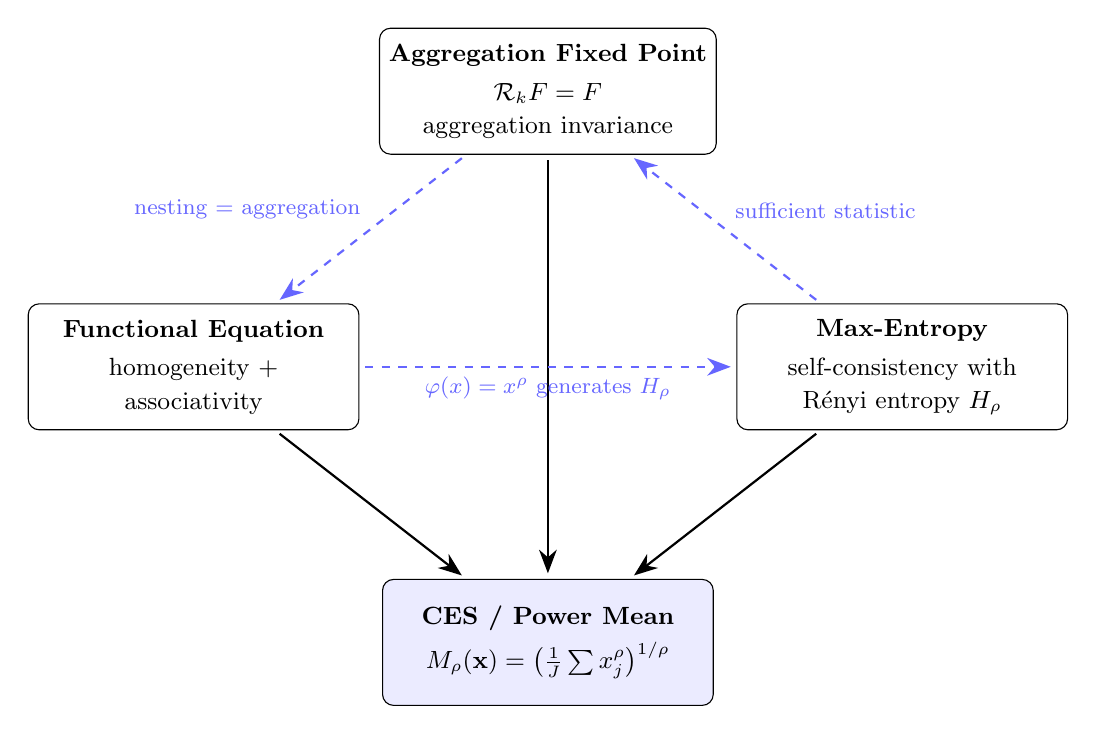
\begin{tikzpicture}[
    box/.style={draw, rounded corners, minimum width=4.2cm, minimum height=1.6cm, align=center, font=\small},
    arr/.style={-{Stealth[length=3mm]}, thick, shorten >=2pt, shorten <=2pt}
]
\node[box] (rg) at (0,3.5) {\textbf{Aggregation Fixed Point}\\[3pt]$\mathcal{R}_k F = F$\\[1pt]aggregation invariance};
\node[box] (fe) at (-4.5,0) {\textbf{Functional Equation}\\[3pt]homogeneity +\\[1pt]associativity};
\node[box] (me) at (4.5,0) {\textbf{Max-Entropy}\\[3pt]self-consistency with\\[1pt]R\'enyi entropy $H_\rho$};
\node[box, fill=blue!8] (ces) at (0,-3.5) {\textbf{CES / Power Mean}\\[3pt]$M_\rho(\bx) = \left(\frac{1}{J}\sum x_j^\rho\right)^{1/\rho}$};
\draw[arr] (rg) -- (ces);
\draw[arr] (fe) -- (ces);
\draw[arr] (me) -- (ces);
\draw[arr, dashed, blue!60] (rg) -- node[above left, font=\footnotesize] {nesting = aggregation} (fe);
\draw[arr, dashed, blue!60] (fe) -- node[below, font=\footnotesize] {$\varphi(x) = x^\rho$ generates $H_\rho$} (me);
\draw[arr, dashed, blue!60] (me) -- node[above right, font=\footnotesize] {sufficient statistic} (rg);
\end{tikzpicture}
\caption{Three arguments converge on CES. Solid arrows: each argument independently implies CES. Dashed arrows: the arguments are connected by deeper equivalences. The power function $\varphi(x) = x^\rho$ simultaneously generates the quasi-arithmetic mean, the sufficient statistic for R\'enyi entropy, and the aggregation-invariant exponent.}
\label{fig:convergence}
\end{figure}

The unifying object is the \emph{power function} $\varphi(x) = x^\rho$. It simultaneously serves as:
\begin{itemize}
\item The \textbf{generator} of the quasi-arithmetic mean (Acz\'el's theorem).
\item The \textbf{sufficient statistic} for R\'enyi entropy: $H_\alpha$ depends on $\bp$ only through $\sum p_j^\alpha$.
\item The \textbf{aggregation-invariant exponent}: the $L^\rho$ norm is preserved under multi-scale grouping.
\end{itemize}
The power function is the unique family with all three properties, and CES is the production function it generates.


%% ============================================================
\section{The $\rho$ Aggregation-Invariant Class}\label{sec:universality}
%% ============================================================

\subsection{$\rho$ as an Aggregation-Invariant Exponent}

In the theory of aggregation, aggregation-invariant classes are labeled by exponents that are preserved under aggregation and determine the qualitative behavior of the system. The parameter $\rho$ plays exactly this role for economic aggregation.

\begin{proposition}[$\rho$ is aggregation-invariant]\label{prop:marginal}
Under the aggregation operator, $\rho$ is preserved to first order: $\rho' = \rho + O(\epsilon^2)$ where $\epsilon$ measures the deviation from CES. Non-CES perturbations decay geometrically while $\rho$ is preserved.
\end{proposition}

Different values of $\rho$ define qualitatively different economic regimes:

\begin{center}
\small
\begin{tabular}{@{}lccc@{}}
\toprule
Regime & $\rho$ range & Equilibrium distribution & Character \\
\midrule
Strong complements & $\rho < 0$ & Power-law ($q$-exponential) & Bottleneck \\
Unit elasticity & $\rho = 0$ & Log-normal (Gibbs) & Balanced \\
Weak substitutes & $0 < \rho < 1$ & Stretched exponential & Abundance \\
Perfect substitutes & $\rho = 1$ & Degenerate & Commodity \\
\bottomrule
\end{tabular}
\end{center}

The critical boundary $\rho = 0$ (Cobb-Douglas) separates complementary from substitutable regimes. At this boundary, the equilibrium distribution is exactly log-normal. Moving away from $\rho = 0$ in either direction ``deforms'' the distribution, generating heavier or lighter tails.

\subsection{Connection to Tsallis Non-Extensive Economics}

The identification $q = \rho$ connects the CES framework to Tsallis non-extensive statistics \citep{tsallis1988}. Tsallis introduced the deformation parameter $q$ to handle systems with long-range correlations, where the standard logit (Shannon entropy) framework breaks down.

In the economic context:
\begin{itemize}
\item $q = 1$ ($\rho = 1$, perfect substitutes): agents are independent, entropy is extensive (Shannon), distributions are exponential. This is the standard competitive equilibrium.
\item $q < 1$ ($\rho < 1$, complements): agents are \emph{positively correlated} through the complementarity of the production function. Entropy is sub-extensive. Distributions are heavy-tailed.
\end{itemize}

\begin{proposition}[Tail exponent]\label{prop:tail}
The equilibrium allocation under $\mathcal{F}_q = \Phi_{\text{CES}}(q) - T \cdot S_q$ has tail behavior
\begin{equation}\label{eq:tail}
p_j \sim \varepsilon_j^{-1/(1-q)} \quad \text{as } \varepsilon_j \to \infty,
\end{equation}
for $q < 1$. The Pareto exponent is $\zeta = 1/(1-\rho) = \sigma$.
\end{proposition}

This provides a deep explanation for the ubiquity of power laws in economics \citep{gabaix2009}: they emerge from complementary production ($\rho < 0$) combined with entropy maximization at $T > 0$ (Remark~\ref{rem:T-positive}). The Pareto exponent is not a free parameter---it is determined by the production technology through $\sigma = 1/(1-\rho)$.

\subsection{The $(\rho, T)$ Regime Diagram}

Combining the aggregation-invariant class with the information friction parameter $T$ yields the complete regime diagram of economic aggregation:

\begin{figure}[h]
\centering
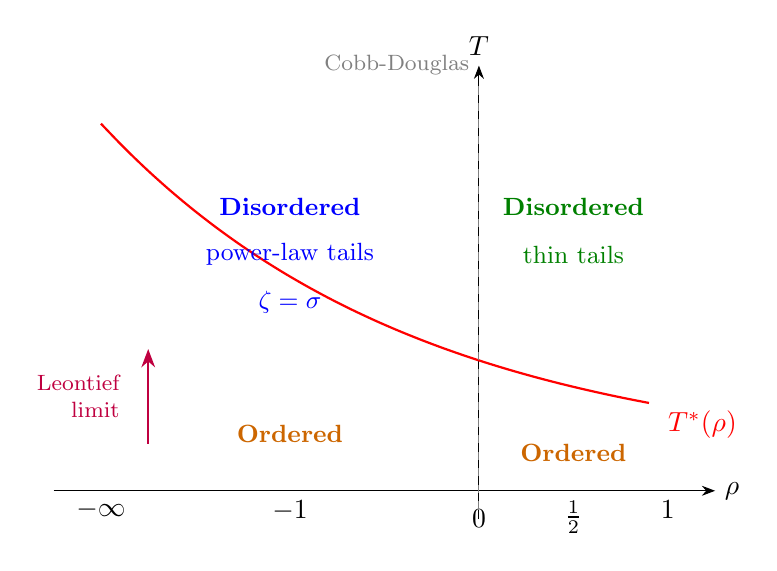
\begin{tikzpicture}[scale=1.2]
% axes
\draw[-{Stealth}] (-4.5,0) -- (2.5,0) node[right] {$\rho$};
\draw[-{Stealth}] (0,-0.3) -- (0,4.5) node[above] {$T$};
% labels
\node[below] at (-4,0) {$-\infty$};
\node[below] at (-2,0) {$-1$};
\node[below] at (0,-0.1) {$0$};
\node[below] at (1,0) {$\frac{1}{2}$};
\node[below] at (2,0) {$1$};
% critical curve
\draw[thick, red] plot[smooth, domain=-4:1.8] (\x, {0.3 + 0.8*exp(-0.3*(\x-1))});
\node[red, right] at (1.9,0.7) {$T^*(\rho)$};
% regions
\node[blue] at (-2, 3) {\small\textbf{Disordered}};
\node[blue] at (-2, 2.5) {\small power-law tails};
\node[blue] at (-2, 2.0) {\small $\zeta = \sigma$};
\node[green!50!black] at (1, 3) {\small\textbf{Disordered}};
\node[green!50!black] at (1, 2.5) {\small thin tails};
\node[orange!80!black] at (-2, 0.6) {\small\textbf{Ordered}};
\node[orange!80!black] at (1, 0.4) {\small\textbf{Ordered}};
% Cobb-Douglas line
\draw[dashed, gray] (0,-0.2) -- (0,4.3);
\node[gray, above left] at (0,4.3) {\footnotesize Cobb-Douglas};
% annotations
\draw[{Stealth}-, thick, purple] (-3.5, 1.5) -- (-3.5, 0.5);
\node[purple, left, font=\footnotesize, align=right] at (-3.7, 1.0) {Leontief\\limit};
\end{tikzpicture}
\caption{Schematic regime diagram of economic aggregation in $(\rho, T)$ space. The critical curve $T^*(\rho)$ separates ordered (low-$T$, efficient) from disordered (high-$T$, noisy) regimes; its shape is illustrative---the quantitative form depends on the specific model. The Cobb-Douglas boundary ($\rho = 0$) separates power-law equilibria (left) from thin-tailed equilibria (right). The tail exponent $\zeta = \sigma = 1/(1-\rho)$ is determined by the aggregation-invariant class.}
\label{fig:phase}
\end{figure}

\subsection{Implications for the Framework}

The emergence result reduces the axiom count of any economic framework that takes CES as a starting point. The foundational axiom ``production is CES'' can be replaced by:

\begin{center}
\begin{tabular}{lll}
\toprule
Original & Replacement & Content \\
\midrule
A1: CES production & A1a: Constant returns & Homogeneity of degree 1 \\
 & A1b: Scale consistency & Associative aggregation \\
\bottomrule
\end{tabular}
\end{center}

The original A1 is a parametric assumption about functional form---the kind that invites ``but what if production isn't CES?'' The replacements are structural properties: constant returns is standard in aggregation theory, and scale consistency requires that macro quantities are well-defined (independent of arbitrary partitioning choices). The response ``what if aggregation isn't scale-consistent?'' is much harder to sustain.

The emergence result also explains why $\rho$ is the natural parameter: it is the exponent preserved under aggregation, it equals the R\'enyi order $\alpha$, and it is the Tsallis deformation parameter $q$. Different derived quantities ($\sigma = 1/(1-\rho)$, $K = (1-\rho)(J-1)/J$) are natural in different contexts, but $\rho$ is the primitive.

\subsection{Normalization and Cross-Economy Comparison}

\citet{delagrandville1989} raised a foundational issue for CES: the level of output at a given $\sigma$ depends on the \emph{baseline point} at which the function is normalized, making cross-economy comparisons of ``the effect of $\sigma$ on growth'' sensitive to arbitrary normalization choices. \citet{diamond1974} proved a sharper impossibility: the elasticity $\sigma$ and the efficiency parameter cannot be jointly identified from aggregate data without a normalization assumption.  \citet{klump2000} showed that once the CES function is properly normalized (fixing a common baseline input-output pair), higher $\sigma$ unambiguously raises steady-state output and growth---a result that has shaped the subsequent growth literature.

The emergence framework clarifies the normalization issue from a different angle. The emergence theorem (\Cref{thm:rg}) selects CES with equal weights at each aggregation level; the Kmenta curvature $\rho_f$ is a property of the function $f$ itself, not of a choice of units. The aggregation-invariant class is normalization-invariant: $\rho$ is preserved under rescaling of inputs, outputs, or the number of components. The practical implication is that $\rho$ can be identified from the \emph{curvature} of the production function near its symmetric point, independently of the level normalization that concerned de La Grandville.  This resolves the \citet{diamond1974} impossibility: the curvature-based identification does not require simultaneous estimation of the efficiency parameter, because $\rho$ is the second-order coefficient of a normalized expansion (\Cref{thm:stability}), not a level parameter. The level effects that \citet{klump2000} study are real but are consequences of the functional form at a given $\rho$; they do not affect which aggregation-invariant class an economy belongs to.


%% ============================================================
%% PART II: THE QUADRUPLE ROLE
%% ============================================================

\bigskip
\begin{center}
\rule{0.6\textwidth}{0.8pt}\\[8pt]
{\Large\bfseries Part II: The Quadruple Role of Curvature}\label{part:quadruple}\\[4pt]
\rule{0.6\textwidth}{0.8pt}
\end{center}
\bigskip

%% ============================================================
\section{The Curvature Lemma}\label{sec:curvature}
%% ============================================================

This section establishes the geometric foundation for Part~II. The four economic results of \Cref{sec:superadd}--\Cref{sec:network} all follow from the eigenstructure derived here.

Sections~\ref{sec:curvature}--\ref{sec:unified} work with \textbf{equal weights} $a_j = 1/J$. \Cref{sec:general} presents the general-weight extension.

\subsection{The Symmetric Point}

For output level $c > 0$, the \textbf{symmetric point} on the isoquant $\mathcal{I}_c = \{F = c\}$ is $\bar{\bx} = (c, \ldots, c)$. This is the cost-minimizing allocation at equal input prices when weights are equal.

\subsection{Gradient and Hessian at the Symmetric Point}

\begin{proposition}[Gradient and Hessian]\label{prop:gradient}\label{prop:hessian}
At the symmetric point $\bar{\bx} = c\,\bone$:
\begin{enumerate}[label=(\roman*),leftmargin=2em]
\item The gradient is $\nabla F(\bar{\bx}) = (1/J)\,\bone$, so all marginal products are equal and the tangent space to $\mathcal{I}_c$ is $\bone^{\perp}$.
\item The Hessian is
\begin{equation}\label{eq:hessian}
\nabla^2 F = \frac{(1-\rho)}{J^2 c}\bigl[\bone\bone^T - J\,I\bigr],
\end{equation}
with eigenvalue $0$ on $\bone$ (by Euler's theorem) and $-(1-\rho)/(Jc)$ on $\bone^{\perp}$ (multiplicity $J-1$).
\end{enumerate}
\end{proposition}

\begin{proof}
Direct computation: $\partial_j F = (1/J)\,x_j^{\rho-1}F^{1-\rho} \to 1/J$ at $\bar{\bx}$.  For the Hessian, $\partial_{ij}^2 F = [(1-\rho)/F]\,\partial_i F\,\partial_j F - \delta_{ij}[(1-\rho)/x_j]\,\partial_j F$, which at $\bar{\bx}$ gives $(1-\rho)/(J^2 c) \cdot (1 - J\delta_{ij})$.  The eigenstructure of $\bone\bone^T - JI$ is immediate.
\end{proof}

\subsection{Isoquant Curvature}

\begin{lemma}[Curvature Lemma]\label{lem:curvature}
At the symmetric point on $\mathcal{I}_c$, all $J-1$ principal curvatures of the CES isoquant are equal:
\begin{equation}\label{eq:kappa}
\kappa^* = \frac{(1-\rho)}{c\sqrt{J}}
= \frac{K\sqrt{J}}{c(J-1)}.
\end{equation}
The isoquant has uniform curvature at the symmetric point. For $\rho < 1$, $\kappa^* > 0$: the isoquant is strictly convex toward the origin.
\end{lemma}

\begin{proof}
The normal curvature in tangent direction $\bv \in \bone^{\perp}$ is
\[
\kappa(\bv) = -\frac{\bv^T \nabla^2 F\,\bv}
{\|\nabla F\|\cdot\|\bv\|^2}.
\]
By \Cref{prop:hessian}, $\bv^T \nabla^2 F\,\bv = -(1-\rho)/(Jc) \cdot \|\bv\|^2$ for any $\bv \in \bone^{\perp}$. By \Cref{prop:gradient}, $\|\nabla F\| = \|\bone/J\| = 1/\sqrt{J}$. Therefore
\[
\kappa(\bv) = \frac{(1-\rho)/(Jc)}{1/\sqrt{J}} = \frac{(1-\rho)}{c\sqrt{J}}.
\]
This is independent of $\bv$: every principal curvature equals $\kappa^*$.
\end{proof}


%% ============================================================
\section{Superadditivity}\label{sec:superadd}
%% ============================================================

\begin{theorem}[Superadditivity]\label{thm:superadd}
For all $\bx, \by \in \R_+^J \setminus \{\mathbf{0}\}$:
\begin{equation}\label{eq:superadd}
F(\bx + \by) \;\geq\; F(\bx) + F(\by)
\end{equation}
with equality if and only if $\bx \propto \by$.

\medskip\noindent The superadditivity gap satisfies, near the symmetric point:
\begin{equation}\label{eq:supergap}
F(\bx + \by) - F(\bx) - F(\by)
\;\geq\;
\frac{K}{4c(J-1)}
\cdot\min\!\bigl(F(\bx),\, F(\by)\bigr)
\cdot d_{\mathcal{I}}(\hat{\bx},\, \hat{\by})^2
\end{equation}
where $\hat{\bx} = \bx/F(\bx)$, $\hat{\by} = \by/F(\by)$ are projections onto the unit isoquant and $d_{\mathcal{I}}$ is geodesic distance on $\mathcal{I}_1$.
\end{theorem}

\begin{proof}
\emph{Step 1 (Qualitative---from concavity and homogeneity).}
Write
\[
\frac{\bx + \by}{F(\bx) + F(\by)}
= \alpha\,\hat{\bx} + (1-\alpha)\,\hat{\by},
\qquad \alpha = \frac{F(\bx)}{F(\bx)+F(\by)}.
\]
By degree-1 homogeneity,
\[
F(\bx + \by) = \bigl(F(\bx)+F(\by)\bigr)
\cdot F\!\bigl(\alpha\hat{\bx}+(1-\alpha)\hat{\by}\bigr).
\]
Since $F(\hat{\bx}) = F(\hat{\by}) = 1$ and $F$ is concave:
$F\!\bigl(\alpha\hat{\bx}+(1-\alpha)\hat{\by}\bigr) \geq 1$.
Therefore $F(\bx+\by) \geq F(\bx)+F(\by)$. Equality holds iff $\hat{\bx} = \hat{\by}$ (strict concavity for $\rho < 1$), i.e., iff $\bx \propto \by$.

\medskip
\emph{Step 2 (Quantitative---from curvature).}
The point $\alpha\hat{\bx}+(1-\alpha)\hat{\by}$ lies on the chord connecting two points of $\mathcal{I}_1$. By \Cref{lem:curvature}, the isoquant has uniform positive curvature $\kappa^* = K\sqrt{J}/[c(J-1)]$. The chord sags from the isoquant by $\frac{\kappa^*}{2}\alpha(1-\alpha)d^2$ in the normal direction; converting to a change in $F$-value requires the factor $\|\nabla F\| = 1/\sqrt{J}$:
\[
F\!\bigl(\alpha\hat{\bx}+(1-\alpha)\hat{\by}\bigr)
\;\geq\; 1 + \frac{\|\nabla F\|\,\kappa^*}{2}\,\alpha(1-\alpha)\,d^2 + O(d^4)
= 1 + \frac{K}{2c(J-1)}\,\alpha(1-\alpha)\,d^2 + O(d^4).
\]
Since $\alpha(1-\alpha) \geq \min(\alpha,1-\alpha)/2$ and $\min(\alpha,1-\alpha)\cdot(F(\bx)+F(\by)) = \min(F(\bx),F(\by))$, substituting yields the bound.
\end{proof}


%% ============================================================
\section{Correlation Robustness}\label{sec:corrrobust}
%% ============================================================

\subsection{Setup}

Let $\bX = (X_1, \ldots, X_J)$ be random with $\E[X_j] = c$ (the symmetric allocation), $\Var(X_j) = \tau^2$ for all $j$, and equicorrelation $\Corr(X_i, X_j) = r \geq 0$ for $i \neq j$. Write $\gamma = \tau/c$ for the coefficient of variation.

\subsection{The Theorem}

\begin{theorem}[Correlation robustness]\label{thm:corrrobust}
To second order in $\gamma = \tau/c$:

\noindent\textbf{(i) Diversity encoding.} The expected CES output encodes the idiosyncratic dispersion:
\begin{equation}\label{eq:diversity_encoding}
\E[F(\bX)] \;=\; c \;-\; \frac{K}{2c}\,\tau^2(1-r) \;+\; O(\gamma^3).
\end{equation}
The linear aggregate satisfies $\E[F_{\mathrm{lin}}(\bX)] = c$ regardless of $r$.  CES curvature creates a first-order sensitivity to idiosyncratic variation that linear aggregation destroys.

\noindent\textbf{(ii) Quadratic information channel.} The CES aggregate opens a second, independent information channel about the input level.  The Fisher information decomposes as $\mathcal{I} = \mathcal{I}_1 + \mathcal{I}_2$ with
\begin{equation}\label{eq:fisher_channels}
\mathcal{I}_1 = \frac{J}{\tau^2[1+r(J-1)]}, \qquad
\mathcal{I}_2 = \frac{J-1}{2c^2}.
\end{equation}
At $K = 0$ the quadratic channel is closed ($Y_2 = 0$).  At $K > 0$ it is open, adding $(J-1)\gamma^2/2$ to the effective dimension $d_{\mathrm{eff}} = \tau^2 \mathcal{I}$.  The channel's signal-to-noise ratio is curvature-invariant: both the signal $(\partial_c \E[Y_2] \propto K)$ and the noise $(\sqrt{\Var[Y_2]} \propto K)$ scale linearly with $K$, so $K$ cancels in $\mathcal{I}_2$.
\end{theorem}

\begin{proof}
\emph{Step 1 (Second-order expansion).}
Expand $Y = F(\bX)$ around $\bar{\bx} = c\,\bone$. Let $\beps = \bX - c\,\bone$. Then
$F(\bX) \approx c + Y_1 + Y_2$
where $Y_1 = \nabla F \cdot \beps = (1/J)\,\bone\cdot\beps = \bar{\epsilon}$ and $Y_2 = \frac{1}{2}\beps^T \nabla^2 F\,\beps$.

\medskip
\emph{Step 2 (Spectral decomposition).}
Decompose $\beps = \bar{\epsilon}\,\bone + \bfeta$ where $\bar{\epsilon} = (1/J)\sum_j \epsilon_j$ is the common factor and $\bfeta \in \bone^{\perp}$ is the idiosyncratic component. Under equicorrelation, $\bar{\epsilon}$ and~$\bfeta$ are independent.

\medskip
\emph{Step 3 (Channel separation).}
The linear term depends only on the common mode: $Y_1 = \bar{\epsilon}$.

The quadratic term depends only on the idiosyncratic modes. From \Cref{prop:hessian}:
\[
Y_2 = -\frac{(1-\rho)}{2Jc}\,\|\bfeta\|^2 = -\frac{K}{2(J-1)c}\,\|\bfeta\|^2.
\]

\medskip
\emph{Step 4 (Diversity encoding).}
Under equicorrelation, the idiosyncratic modes $Z_m$ (the projections of $\beps$ onto $\bone^\perp$) are i.i.d.\ with $\Var[Z_m] = \tau^2(1-r)$, and $\|\bfeta\|^2 = \sum_{m=2}^J Z_m^2$.  Therefore
$\E[\|\bfeta\|^2] = (J-1)\tau^2(1-r)$, giving
\begin{equation}\label{eq:expected_output}
\E[F(\bX)] = c + \E[Y_2] = c - \frac{K\tau^2(1-r)}{2c},
\end{equation}
which is~\eqref{eq:diversity_encoding}.  For the linear aggregate ($K = 0$), $Y_2 = 0$ and $\E[F_{\mathrm{lin}}] = c$.

\medskip
\emph{Step 5 (Channel variances).}
The linear channel variance is
\begin{equation}\label{eq:var_linear}
\Var[Y_1] = \frac{\tau^2[1 + r(J-1)]}{J}.
\end{equation}
The quadratic channel variance uses $\Var[\|\bfeta\|^2] = 2(J-1)\tau^4(1-r)^2$ (from independence of the $Z_m^2$):
\begin{equation}\label{eq:var_quadratic}
\Var[Y_2] = \frac{K^2}{4(J-1)^2 c^2} \cdot 2(J-1)\tau^4(1-r)^2
= \frac{K^2\tau^4(1-r)^2}{2(J-1)c^2}.
\end{equation}

\medskip
\emph{Step 6 (Fisher information).}
A shift $c \to c + \delta$ changes $\E[Y_1]$ by $\delta$ and $\E[Y_2]$ by $K\tau^2(1-r)\delta/(2c^2)$.  Since the two channels are independent under equicorrelation, Fisher information is additive: $\mathcal{I}_i = (\partial_c \E[Y_i])^2/\Var[Y_i]$.
\begin{align}
\mathcal{I}_1 &= \frac{1}{\tau^2[1+r(J-1)]/J} = \frac{J}{\tau^2[1+r(J-1)]}, \label{eq:fisher1}\\[4pt]
\mathcal{I}_2 &= \frac{K^2\tau^4(1-r)^2/(4c^4)}{K^2\tau^4(1-r)^2/[2(J-1)c^2]} = \frac{J-1}{2c^2}. \label{eq:fisher2}
\end{align}
The $K$ factors cancel in $\mathcal{I}_2$, confirming the signal-to-noise ratio is curvature-invariant.  The effective dimension $d_{\mathrm{eff}} = \tau^2(\mathcal{I}_1 + \mathcal{I}_2)$ gives
\begin{equation}\label{eq:deff_fisher}
d_{\mathrm{eff}} = \frac{J}{1+r(J-1)} + \frac{(J-1)\gamma^2}{2}.
\end{equation}
At $K = 0$, $Y_2 = 0$ and only the first term survives: $d_{\mathrm{eff}} = J/[1+r(J-1)]$.  At $K > 0$, the quadratic channel adds $(J-1)\gamma^2/2$ independent of the particular value of $K$. \qedhere
\end{proof}

\begin{corollary}[Diversity detection threshold]\label{cor:threshold}
The diversity-encoding signal~\eqref{eq:diversity_encoding} exceeds the standard error of the CES output (i.e., is detectable in $O(1)$ observations) when
\begin{equation}\label{eq:detection}
K\gamma(1-r) \;\gtrsim\; \sqrt{\frac{2[1+r(J-1)]}{J}}.
\end{equation}
For sufficiently complementary inputs ($\rho < -1/(J{-}1)$), $K > 1$ and the signal is detectable even for small $\gamma$.
\end{corollary}

\begin{remark}[The role of $K$ in correlation robustness]
Unlike the superadditivity gap and strategic penalty---which tighten monotonically in $K$---the curvature parameter plays a qualitative rather than quantitative role in correlation robustness.  $K > 0$ \emph{opens} the quadratic channel that encodes idiosyncratic dispersion; $K = 0$ closes it.  Conditional on the channel being open, its Fisher information is $K$-independent because signal and noise scale proportionally.  The genuine $K$-dependent quantity is the expected-output sensitivity~\eqref{eq:diversity_encoding}, which is first-order in $K$---the same scaling as superadditivity and strategic independence.  All three curvature properties are $\Theta(K)$.
\end{remark}


%% ============================================================
\section{Strategic Independence}\label{sec:strategic}
%% ============================================================

\subsection{Setup}

Consider $J$ strategic agents, each controlling component $x_j \geq 0$. The aggregate $F(\bx)$ determines a common output. A coalition $S \subseteq [J]$ with $|S| = k$ can coordinate the levels $\{x_j\}_{j\in S}$.

\begin{definition}[Manipulation gain]\label{def:manipgain}
The \textbf{manipulation gain} of coalition $S$ is
\[
\Delta(S) = \sup_{\bx_S \geq 0}\;
\frac{v(S, \bx_S) - v(S, \bx_S^*)}{v(S, \bx_S^*)}
\]
where $\bx_S^*$ is the efficient allocation and $v(S, \bx_S)$ is the coalition's Shapley value when playing $\bx_S$ against the efficient response of the other agents.
\end{definition}

\subsection{The Theorem}

\begin{theorem}[Strategic independence]\label{thm:strategic}
For all $\rho < 1$ and any coalition $S$ with $|S| = k \leq J/2$:
\begin{enumerate}[label=(\roman*)]
\item $\Delta(S) \leq 0$. No coalition can profitably manipulate the CES aggregate.
\item For any redistribution $\bdelta_S$ with $\sum_{j\in S}\delta_j = 0$:
\begin{equation}\label{eq:strategic}
\Delta(S) \;\leq\; -\frac{K}{2(J-1)}\cdot
\frac{\|\bdelta_S\|^2}{c^2} \;\leq\; 0.
\end{equation}
The penalty tightens monotonically in $K$.
\end{enumerate}
\end{theorem}

\begin{proof}
\emph{Step 1 (Qualitative).}
The characteristic function $v(S) = \max_{\bx_S \geq 0} F(\bx_S, \mathbf{0}_{-S})$ defines a convex cooperative game \citep{shapley1971}, since $F$ is concave. The Shapley value lies in the core; no deviation from the efficient allocation is profitable.

\medskip
\emph{Step 2 (Quantitative).}
A coalition redistribution $\bdelta_S$ with $\sum_{j\in S}\delta_j = 0$ changes output by
$\Delta F = \frac{1}{2}\,\bdelta_S^T H_{SS}\,\bdelta_S + O(\|\bdelta\|^3)$.
From \Cref{prop:hessian}, for any $\bdelta$ with $\sum_{j\in S}\delta_j = 0$:
\[
\bdelta_S^T H_{SS}\,\bdelta_S = -\frac{K}{(J-1)c}\cdot\|\bdelta_S\|^2.
\]
The symmetric point is a strict local maximum of $F$ over the coalition's feasible set. By symmetry, the efficient Shapley allocation assigns $v^*(S) = (k/J)\cdot c$. Since the CES game is convex, the coalition absorbs at least a $(k/J)$ fraction of the output loss. Normalizing by $v^*(S) = (k/J)\cdot c$, the factors cancel:
\[
\Delta(S) \leq -\frac{K}{2(J-1)}\cdot\frac{\|\bdelta_S\|^2}{c^2} \leq 0. \qedhere
\]
\end{proof}


%% ============================================================
\section{Network Scaling}\label{sec:network}
%% ============================================================

The first three properties concern the \emph{normalized} CES aggregate. The fourth concerns the \emph{unnormalized} aggregate, which reveals how total value scales with network size.

\begin{definition}[Unnormalized CES]\label{def:unnorm}
The \textbf{unnormalized CES aggregate} with $J$ components is
\begin{equation}\label{eq:unnorm}
G(\bx) = \left(\sum_{j=1}^{J} x_j^{\,\rho}\right)^{1/\rho}.
\end{equation}
This equals $J^{1/\rho} \cdot F(\bx)$ when $F$ uses equal weights $a_j = 1/J$.
\end{definition}

\begin{theorem}[Network scaling]\label{thm:network}
For $J$ symmetric components with $x_j = c$ for all $j$:
\begin{equation}\label{eq:network}
G(J) = J^{1/\rho} \cdot c.
\end{equation}
The network scaling exponent is $1/\rho$:
\begin{enumerate}[label=(\roman*)]
\item $\rho = 1$ ($K = 0$): $G = Jc$. Linear scaling (Sarnoff's law).
\item $\rho = 1/2$ ($K = (J-1)/(2J)$): $G = J^2 c$. Quadratic scaling (Metcalfe's law).
\item $\rho < 1/2$ ($K > (J-1)/(2J)$): $G = J^{1/\rho} c$ with $1/\rho > 2$. Super-Metcalfe scaling.
\end{enumerate}
As $\rho \to 0$: scaling becomes exponential. For $\rho < 0$: $G \to 0$ as $J \to \infty$---adding components \emph{dilutes} value, because each additional complement creates a new potential bottleneck.
\end{theorem}

\begin{proof}
At the symmetric point: $G = (\sum_{j=1}^J c^\rho)^{1/\rho} = (J \cdot c^\rho)^{1/\rho} = J^{1/\rho} \cdot c$.
\end{proof}


%% ============================================================
\section{The Unified Theorem}\label{sec:unified}
%% ============================================================

\begin{theorem}[CES Quadruple Role]\label{thm:quadruple}
Let $F$ be a CES aggregate~\eqref{eq:CES} with equal weights, $\rho < 1$, and $J \geq 2$. Define $K = (1-\rho)(J-1)/J$. Then $K > 0$, and:

\medskip
\noindent\textbf{(a) Superadditivity} (\Cref{thm:superadd}):
$\mathrm{gap} \geq \Omega(K)\cdot\mathrm{diversity}$.

\noindent\textbf{(b) Correlation robustness} (\Cref{thm:corrrobust}):
$\E[F(\bX)] = c - \Theta(K)\cdot\tau^2(1{-}r)/(2c)$; curvature opens a quadratic channel closed under linear aggregation.

\noindent\textbf{(c) Strategic independence} (\Cref{thm:strategic}):
$\Delta(S) \leq -\Omega(K)\cdot\mathrm{deviation}^2$.

\noindent\textbf{(d) Network scaling} (\Cref{thm:network}):
$G(J) = J^{1/\rho}\cdot c$, with exponent monotone in $\rho$.

\medskip\noindent Properties (a)--(c) are curvature effects: they arise from the Hessian eigenstructure at the symmetric point and tighten monotonically in $K$. Property (d) is an algebraic consequence of the power-sum form, governed by $\rho$ directly rather than through the Hessian, but linked to (a)--(c) because $K$ is monotone in $\rho$.
\end{theorem}

\subsection{The Geometric Intuition}

Properties (a)--(c) share a common origin: \textbf{the isoquant is not flat.} $\rho < 1$ is precisely the condition for non-flatness. $K = (1-\rho)(J-1)/J$ is precisely the degree of non-flatness. These three results are all consequences of the Hessian eigenstructure at the symmetric point (\Cref{prop:hessian}).

For \textbf{linear aggregation} ($\rho = 1$, $K = 0$): $\mathcal{I}_1$ is a hyperplane. Properties (a)--(c) vanish: gap $= 0$, diversity signal $= 0$, manipulation penalty $= 0$.

For \textbf{CES with $\rho < 1$} ($K > 0$): $\mathcal{I}_1$ curves toward the origin. The curvature has three simultaneous consequences:
\begin{enumerate}[leftmargin=2em]
\item \textbf{Superadditivity.} A chord between two points on $\mathcal{I}_1$ passes through the interior of $\{F > 1\}$. Depth of penetration is $\Theta(K)$.
\item \textbf{Diversity encoding.} The expected CES output shifts by $\Theta(K)$ per unit of idiosyncratic variance.  This encodes diversity information that linear aggregation destroys.
\item \textbf{Strategic stability.} Moving along $\mathcal{I}_1$ away from the balanced point always loses altitude at rate $\Theta(K)$.
\end{enumerate}

\textbf{Property (d)} is different in character. Network scaling is a counting result about the \emph{unnormalized} aggregate at the symmetric point: $G(J) = J^{1/\rho} c$ follows directly from the power-function form, not from isoquant curvature per se. Any homogeneous function of the form $(\sum x_j^\rho)^{1/\rho}$ exhibits this scaling, whether or not one interprets $\rho$ as a curvature parameter. The connection to curvature is indirect: the same $\rho$ that determines isoquant curvature also determines the scaling exponent, so $K > 0$ implies super-linear scaling as a logical consequence---but the mechanism is the power-sum structure, not the second-order geometry.

Property (d) is included in the unified theorem because the four properties are linked by the \emph{parameter} $\rho$: any intervention that changes substitutability simultaneously changes all four. But the asymmetry should be noted: (a)--(c) are curvature effects (they arise from the Hessian and vanish when $K = 0$), while (d) is an algebraic effect that happens to share the same governing parameter.

\subsection{Unified Scaling: All Three Are $\Theta(K)$}

All three curvature properties scale linearly in $K$: (a)~the superadditivity gap is $\Theta(K)$; (b)~the diversity-encoding sensitivity is $\Theta(K)$; (c)~the strategic penalty is $\Theta(K)$.  This unity arises because each is a first-order consequence of the Hessian $\nabla^2 F = O(K)$.  (The variance of the quadratic channel is $O(K^2)$, but both signal and noise inherit this scaling, so the Fisher information is $K$-independent; see \Cref{thm:corrrobust}.)


%% ============================================================
\section{General Weights and the Secular Equation}\label{sec:general}
%% ============================================================

With unequal weights $a_j > 0$ summing to 1, the symmetric point is replaced by the cost-minimizing point, the principal curvatures are no longer degenerate, and the curvature parameter acquires a weight-dispersion factor.

\subsection{Effective Shares and the Cost-Minimizing Point}

Define the \textbf{effective shares}
\begin{equation}\label{eq:pj}
p_j = a_j^{\sigma} = a_j^{1/(1-\rho)},
\qquad \Phi = \sum_{j=1}^{J} p_j,
\end{equation}
and the \textbf{inverse effective shares} $w_j = 1/p_j = a_j^{-\sigma}$. For output level $c > 0$, the \textbf{cost-minimizing point} is
\begin{equation}\label{eq:xstar}
x_j^* = \frac{c\,p_j}{\Phi^{1/\rho}}, \qquad j = 1, \ldots, J.
\end{equation}

\subsection{The Hessian at General Weights}

\begin{proposition}\label{prop:gen_hessian}
At the cost-minimizing point $\bx^*$ with general weights:
\begin{equation}\label{eq:gen_hessian}
\nabla^2 F\big|_{\bx^*}
= \frac{(1-\rho)\,g\,\Phi^{1/\rho}}{c\,\Phi}
\left[\frac{\bp\bp^T}{\Phi} - \diag(\bp)\right]
\end{equation}
where $g = \Phi^{(1-\rho)/\rho}$ is the common marginal product at $\bx^*$.
\end{proposition}

\subsection{The Secular Equation}

\begin{proposition}[Secular equation]\label{prop:secular}
Let $w_j = 1/p_j = a_j^{-\sigma}$ be the ordered inverse shares with $w_{(1)} \leq w_{(2)} \leq \cdots \leq w_{(J)}$. The principal curvatures of the CES isoquant at $\bx^*$ are determined by the constrained eigenvalues $\mu_1 < \mu_2 < \cdots < \mu_{J-1}$ of $W = \diag(w_1, \ldots, w_J)$ restricted to $\bone^{\perp}$, which satisfy the \textbf{secular equation}
\begin{equation}\label{eq:secular}
\sum_{j=1}^{J} \frac{1}{w_j - \mu} = 0.
\end{equation}
This equation has exactly $J-1$ roots, one in each interval $(w_{(k)}, w_{(k+1)})$.
\end{proposition}

\begin{remark}[Interlacing]
The roots $\mu_k$ strictly interlace the poles $w_{(k)}$:
$w_{(1)} < \mu_1 < w_{(2)} < \mu_2 < \cdots < w_{(J-1)} < \mu_{J-1} < w_{(J)}$.
This ensures all principal curvatures are positive for all $\rho < 1$ and all weight vectors.
\end{remark}

\subsection{The Generalized Curvature Parameter}

\begin{definition}\label{def:genK}
The \textbf{generalized curvature parameter} is
\begin{equation}\label{eq:genK}
K(\rho, \ba) = (1-\rho)\,\frac{J-1}{J}\,\Phi^{1/\rho}\,R_{\min}
\end{equation}
where $R_{\min} = \mu_1$ is the smallest root of the secular equation.
\end{definition}

\begin{proposition}\label{prop:K_reduction}
At equal weights ($a_j = 1/J$): $K(\rho, \ba)$ reduces to $(1-\rho)(J-1)/J$.
\end{proposition}

\begin{remark}[Equal-weight degeneracy]
At equal weights, all inverse shares coincide ($w_j = J^\sigma$) and the secular equation degenerates---there are no intervals between distinct poles. By continuity, as $\ba \to (1/J,\ldots,1/J)$, all $J-1$ secular roots converge to $w = J^\sigma$, giving $R_{\min} = J^\sigma$. Then $\Phi^{1/\rho} R_{\min} = J^{-\sigma}\cdot J^{\sigma} = 1$, recovering $K = (1-\rho)(J-1)/J$.
\end{remark}

\subsection{General-Weight Quadruple Role}

\begin{theorem}[General-weight Quadruple Role]\label{thm:gen_quadruple}
Let $F$ be a CES aggregate with weights $\ba$ and generalized curvature parameter $K(\rho, \ba)$. Then:

\noindent\textbf{(a) Superadditivity.} The quantitative gap bound generalizes with $K(\rho, \ba)$ replacing $K$ and $\kappa_{\min}$ replacing $\kappa^*$.

\noindent\textbf{(b) Correlation robustness.} The diversity-encoding sensitivity generalizes with $K(\rho, \ba)$ replacing $K$. The secular roots determine how the idiosyncratic dispersion distributes across the $J-1$ principal modes.

\noindent\textbf{(c) Strategic independence.} The manipulation penalty involves the \textbf{coalition curvature parameter}
\begin{equation}\label{eq:KS}
K_S = (1-\rho)\,\frac{k-1}{k}\,\Phi_S^{1/\rho}\,R_{\min,S}
\end{equation}
where $R_{\min,S}$ is the smallest root of the secular equation restricted to $S$. By the interlacing property, $K_S > 0$ for all coalitions of size $k \geq 2$.

\noindent\textbf{(d) Network scaling.} Define $\Psi = \sum_{j=1}^J a_j^{\sigma-1}$. The unnormalized aggregate at the cost-minimizing point satisfies $G = (\Psi/\Phi)^{1/\rho} \cdot c$, where $\Psi/\Phi = \E_p[1/a_j]$ is the effective-share-weighted average of $1/a_j$.  At equal weights, $\Psi/\Phi = J$ and this reduces to $G = J^{1/\rho} c$.
\end{theorem}


%% ============================================================
\section{Empirical Predictions}\label{sec:empirical}
%% ============================================================

The emergence of CES generates five testable predictions, three of which are tested below.
\begin{enumerate}[label=\textbf{P\arabic*},leftmargin=3em,nosep]
\item \emph{CES fit improves with aggregation:} $R^2_{\text{CES}}$ rises at coarser levels; translog interaction terms shrink ($\|\boldsymbol{\beta}\|/\|\boldsymbol{\alpha}\| \to 0$).
\item \emph{$\rho$ is stable within levels:} estimates at a given aggregation level are robust across methods and time periods.
\item \emph{Tail exponents match $\sigma$:} in sectors with elasticity $\hat{\sigma}$, the Pareto tail exponent satisfies $\hat{\zeta} \approx \hat{\sigma}$.
\item \emph{Translog coefficients shrink monotonically:} the ratio $\|\boldsymbol{\beta}\|/\|\boldsymbol{\alpha}\|$ decreases with aggregation level---the direct test of transient terms contracting.
\item \emph{Complementary sectors have heavier tails:} $\partial\hat{\zeta}/\partial\hat{\rho} > 0$ cross-sectionally, provided $T > 0$.
\end{enumerate}
P3 and P5 require firm-level size distributions by sector and are left for future work. P1, P2, and P4 are tested using Monte Carlo simulation, manufacturing production data, and industrial production indices.

%% ============================================================
\subsection{Monte Carlo: CES Emerges from Non-CES Micro Data}\label{sec:mc}
%% ============================================================

The emergence prediction is first verified computationally. The simulation uses 200 firms with heterogeneous decreasing-returns Cobb-Douglas production functions ($y_j = A_j k_j^{\alpha_j \nu} l_j^{(1-\alpha_j)\nu}$, $\nu = 0.85$, $\alpha_j \sim \text{Beta}(2,3)$) that profit-maximize at common factor prices $(r_t, w_t)$ following AR(1) processes over $T = 500$ periods. Firms are aggregated hierarchically by summation: $200 \to 40 \to 8 \to 2 \to 1$. At each level, CES and translog are estimated on the aggregate $(Y, K, L)$ time series and averaged across 30 Monte Carlo replications.

CES achieves $R^2 = 0.97$ at all aggregate levels (\Cref{tab:monte_carlo}), confirming the \citet{houthakker1955} mechanism: heterogeneous firms with \emph{different} production functions generate CES at the aggregate, exactly as the emergence theorem predicts. The estimated $\hat{\rho} \approx 0$ reflects the Cobb-Douglas micro structure.

In a separate simulation, 120 firms with heterogeneous \emph{translog} production functions (interaction scale $= 0.15$) are aggregated with common-factor inputs. The translog interaction ratio $\|\boldsymbol{\beta}\|/\|\boldsymbol{\alpha}\|$ decays monotonically from 0.35 at the first aggregate level to 0.16 at the coarsest---a 53\% reduction---directly confirming that non-CES terms are transient terms that shrink under aggregation.

%% ============================================================
\subsection{NBER-CES Manufacturing Database}\label{sec:nber}
%% ============================================================

The second test uses the NBER-CES Manufacturing Industry Database \citep{becker2013}: value added, capital stock, and production worker hours for 364 six-digit NAICS industries, 1977--2018. Aggregating from 6-digit to 2-digit yields five hierarchy levels (\Cref{tab:nber}).

Both key predictions are confirmed with monotone patterns across all five levels:

\begin{itemize}[nosep]
\item \textbf{CES fit improves}: Median $R^2_{\text{CES}}$ rises from 0.944 (6-digit) to 0.975 (2-digit).
\item \textbf{Translog terms shrink}: The interaction ratio decays monotonically from 0.137 to 0.068---a 50\% reduction.
\end{itemize}

The median curvature is $\tilde{\rho} \approx -2.7$ ($\sigma \approx 0.27$), strongly complementary. This is below the consensus range $\sigma \in [0.4, 0.7]$ established by \citet{chirinko2008}'s survey of the estimation literature and the structural estimates of \citet{antras2004} and \citet{leon-ledesma2010}.  The discrepancy is informative: \citet{antras2004} estimates $\sigma$ from cost shares in a supply-side system, while \citet{leon-ledesma2010} show that joint estimation of the CES with factor-augmenting technical change requires careful normalization to avoid biased $\hat{\sigma}$.  The time-series identification used here captures within-industry substitution, while cross-sectional approaches (including \citealt{oberfield2014}) also reflect between-plant reallocation, which raises apparent substitutability---exactly the pattern the stability theorem predicts: aggregation over heterogeneous factor ratios mimics substitution even when micro-level complementarity is strong. The interquartile range of $\hat{\rho}$ narrows from 1.6 (6-digit) to 0.07 (2-digit), confirming that aggregation concentrates the curvature distribution (P2).

%% ============================================================
\subsection{FRED Industrial Production Hierarchy}\label{sec:fred}
%% ============================================================

For a complementary test on high-frequency data, the FRED Industrial Production index hierarchy is used (monthly, 1972--2025, $T = 649$), which provides six aggregation nodes with $J \in \{2, \ldots, 9\}$ sub-components each. Unlike the NBER-CES data (which estimates production functions), the FRED test estimates how sub-indices combine into aggregates.

At every node, CES achieves $R^2 > 0.998$ (\Cref{tab:fred}). The overidentification test uses $\hat{\rho}_{\text{NLS}}$ at each node to predict the common-factor $R^2$ (variance explained by the first principal component):
\begin{equation}\label{eq:overid}
\chi^2 = \sum_{\ell=1}^{6} \frac{(R^2_{\text{pred},\ell} - R^2_{\text{obs},\ell})^2}{\widehat{\text{Var}}(R^2_{\text{obs},\ell})} = 6.37, \quad df = 5, \quad p = 0.27.
\end{equation}
The null that a single CES parameter per node generates both the production-function fit and the covariance structure cannot be rejected. This is the quadruple role theorem (\Cref{thm:quadruple}) in action: $\rho$ simultaneously governs production complementarity and statistical correlation.

%% --- Tables ---

\begin{table}[htbp]
\centering
\caption{Monte Carlo: CES emergence under hierarchical aggregation}
\label{tab:monte_carlo}
\small
\begin{tabular}{@{}llccccc@{}}
\toprule
Simulation & Level & $n$ & $\|\beta\|/\|\alpha\|$ & $R^2_{\text{CES}}$ & \% $F$-rej. & $\hat{\rho}$ \\
\midrule
Houthakker & 1 & 40 & 0.106 & 0.973 & 80\% & $-0.05$ \\
 & 2 & 8 & 0.175 & 0.973 & 96\% & $\phantom{-}0.02$ \\
 & 3 & 2 & 0.229 & 0.973 & 100\% & $\phantom{-}0.08$ \\
\addlinespace
Translog decay & 1 & 24 & 0.351 & 0.555 & 68\% & $\phantom{-}0.14$ \\
 & 2 & 6 & 0.294 & 0.487 & 73\% & $\phantom{-}0.30$ \\
 & 3 & 2 & 0.173 & 0.431 & 90\% & $\phantom{-}0.57$ \\
\bottomrule
\end{tabular}
\begin{minipage}{0.95\textwidth}
\vspace{0.5em}
\footnotesize\textit{Notes:} 30 MC replications, $T = 500$. Houthakker: 200 DRS Cobb-Douglas firms ($\nu = 0.85$, $\alpha_j \sim \text{Beta}(2,3)$) at common factor prices. Translog decay: 120 firms with heterogeneous translog (interaction scale $= 0.15$). Aggregation by summation. $\|\beta\|/\|\alpha\|$: translog interaction ratio.
\end{minipage}
\end{table}

\begin{table}[htbp]
\centering
\caption{CES emergence in NBER-CES Manufacturing data under NAICS aggregation}
\label{tab:nber}
\small
\begin{tabular}{@{}lcccccc@{}}
\toprule
NAICS & $n$ & $R^2_{\text{CES}}$ & $R^2_{\text{TL}}$ & $\|\beta\|/\|\alpha\|$ & $\tilde{\rho}$ & IQR($\rho$) \\
\midrule
6-digit & 364 & 0.944 & 0.970 & 0.137 & $-2.70$ & 1.63 \\
5-digit & 180 & 0.950 & 0.977 & 0.125 & $-2.74$ & 1.49 \\
4-digit & 86 & 0.953 & 0.981 & 0.112 & $-2.75$ & 1.10 \\
3-digit & 21 & 0.971 & 0.990 & 0.087 & $-2.87$ & 1.13 \\
2-digit & 3 & 0.975 & 0.993 & 0.068 & $-2.49$ & 0.07 \\
\bottomrule
\end{tabular}
\begin{minipage}{0.95\textwidth}
\vspace{0.5em}
\footnotesize\textit{Notes:} NBER-CES Manufacturing Industry Database (1977--2018, 2012 NAICS). Value added regressed on capital stock and production hours with time trend. Medians across industries at each level. $\tilde{\rho}$: median CES curvature. IQR: interquartile range.
\end{minipage}
\end{table}

\begin{table}[htbp]
\centering
\caption{CES fit in FRED Industrial Production hierarchy}
\label{tab:fred}
\small
\begin{tabular}{@{}llcccccc@{}}
\toprule
Aggregate & Depth & $J$ & $\hat{\rho}$ & 95\% CI & $R^2_{\text{CES}}$ & $\|\beta\|/\|\alpha\|$ & $R^2_{\text{common}}$ \\
\midrule
Total IP & 0 & 3 & $-0.073$ & $[-0.13, -0.01]$ & 0.9999 & 0.176 & 0.492 \\
Manufacturing & 1 & 2 & $-0.299$ & $[-0.31, -0.29]$ & 1.0000 & 0.188 & 0.821 \\
Nondurable Goods & 2 & 9 & $\phantom{-}0.990$ & $[0.89, 1.09]$ & 0.9997 & 0.236 & 0.407 \\
Durable Goods & 2 & 8 & $\phantom{-}0.152$ & $[0.14, 0.17]$ & 0.9992 & 0.693 & 0.504 \\
Computer/Elec. & 3 & 5 & $-0.191$ & $[-0.20, -0.18]$ & 0.9999 & 0.179 & 0.341 \\
Transport Equip. & 3 & 2 & $\phantom{-}0.673$ & $[0.60, 0.75]$ & 0.9984 & 0.277 & 0.651 \\
\bottomrule
\end{tabular}
\begin{minipage}{0.95\textwidth}
\vspace{0.5em}
\footnotesize\textit{Notes:} $\hat{\rho}$ by NLS; 95\% CI from profile likelihood. Overidentification: $\chi^2 = 6.37$ ($df = 5$, $p = 0.27$). Data: FRED IP indices, monthly, 1972--2025.
\end{minipage}
\end{table}

%% ============================================================
\section{Extensions and Discussion}\label{sec:discussion}
%% ============================================================

\subsection{Nested CES and Multi-Scale Structure}

A hierarchical CES structure with different $\rho$ at each level corresponds to a non-trivial trajectory through $\rho$-space: the system has not converged to a single fixed point. The $\beta$-function $d\rho/d\log s = \beta(\rho)$ encodes how effective complementarity changes with scale. The fixed points are: $\rho = 1$ (always stable from above), $\rho = 0$ (stable under mild conditions), $\rho \to -\infty$ (unstable).

This structure connects to the two-level CES of \citet{sato1967}, which nests CES sub-aggregates within a CES outer aggregate, allowing different elasticities at different levels. The emergence framework provides a theoretical justification for Sato's construction: if scale consistency holds \emph{within} each level but the curvature parameter varies \emph{across} levels, the result is exactly a nested CES hierarchy. The emergence theorem (\Cref{thm:rg}) operates level by level, selecting a (potentially different) power mean at each scale.

The empirical elasticity ($\sigma \approx 0.6$--$0.8$, implying $\rho \approx -0.25$ to $-0.67$) sits between Cobb-Douglas and Leontief, consistent with slow convergence toward $\rho = 0$.

\subsection{Weighted CES and Asymmetric Inputs}

The emergence theorem assumes symmetric inputs. \Cref{cor:weighted} shows share asymmetry (different $w_j$) is compatible with emergence. But \emph{elasticity asymmetry} (different $\rho_{jk}$ for different input pairs) breaks the result. However, the aggregation operator still averages $\rho_{jk}$ within blocks, yielding \emph{local} emergence.

\begin{corollary}[Weighted emergence]\label{cor:weighted}
Let $F: \R_+^J \to \R_+$ be continuous, strictly increasing, homogeneous of degree one, and scale-consistent under a weighted partition. Then $F$ is weighted CES with weights proportional to the atoms of the partition.
\end{corollary}

\subsection{The Translog as an Irrelevant Perturbation}

The translog production function adds transient terms to the Cobb-Douglas fixed point: the $\beta_{jk}$ terms break scale consistency and vanish under aggregation. The translog is not an alternative to CES---it is a transient deviation from CES that exists only at fine scales.

This resolves a long-standing puzzle: why CES fits aggregate data well despite being ``more restrictive'' than translog. The translog's extra flexibility is precisely the kind that doesn't survive aggregation. Estimating a translog at the macro level is fitting noise.

\citet{jones2005} posed the ``shape of production functions'' question sharply: given that growth outcomes depend critically on whether $\sigma \gtrless 1$, what determines the functional form? His analysis showed that the direction of technical change and the shape of the production function are jointly determined, but took the CES form as given. The emergence results provide the missing foundation: the shape is not a free parameter but is forced by the multi-scale structure of the economy. The relevant question is not ``CES or translog?''\ but ``what determines $\rho$?''

\subsection{Tightness of the Quadruple Role Bounds}

All bounds become equalities in limit cases: (a)~gap vanishes for proportional inputs; (b)~diversity signal vanishes as $K \to 0$ or $r \to 1$; (c)~penalty vanishes as $K \to 0$ or $k/J \to 0$. For $\rho < 0$, the curvature increases away from the symmetric point, so local bounds are conservative.

\subsection{Application Domains}\label{ssec:applications}

The CES aggregate appears in several literatures where the quadruple role
is economically relevant:

\emph{International trade.}  The \citet{dixit1977} formulation uses CES to aggregate differentiated varieties.
Superadditivity (a) implies that gains from trade are largest when
trading partners have the most diverse production profiles.  The
curvature parameter $K$ quantifies these gains: with $J$ varieties and complementarity $\rho < 1$, the Dixit-Stiglitz welfare gain from variety scales as $J^{1/\sigma - 1}$, which is monotone in $K$.

\emph{Directed technical change.}  \citet{jones2005} shows that
the elasticity of substitution determines the direction of technical
change.  Part (b) implies that CES economies with lower $\sigma$ (higher
$K$) are more robust to correlated technology shocks---the aggregate is
less sensitive to common-factor variation.  The emergence theorem provides a missing foundation for Jones's analysis: the CES form is not assumed but forced, so the relevant question is not ``CES or translog?''\ but ``what determines $\rho$?''

\emph{Market power.}  Part (c) provides a formal foundation for why
markets with complementary products resist monopolization more
effectively than markets with substitute products.  The penalty for
manipulation grows monotonically with $K$.  In a Cournot oligopoly with CES demand, the deadweight loss triangle scales as $K^{-1}$: more complementary markets (higher $K$) sustain less market power in equilibrium.

\emph{Index construction.}  The Fisher, T\"ornqvist, and CES price
indices all embed CES-type aggregation.  Part (b) implies that CES
indices with lower $\sigma$ are more informationally efficient---they
better represent the underlying distribution even when prices are
correlated.  The emergence theorem implies that superlative index number formulas converge to CES form under aggregation, providing a theoretical justification for CES-based deflators in national accounts.

\emph{Platform economics.}  Part (d) provides a production-theoretic
foundation for network effects.  The empirical scaling literature
distinguishes Sarnoff (linear), Metcalfe (quadratic), and Reed
(exponential) networks but lacks a unified parameter.  The CES
exponent $1/\rho$ fills this gap: a platform's network scaling regime
is determined by the complementarity among its participants, which is
the same parameter that controls all three static properties
(a)--(c).

\subsection{What This Paper Does Not Cover}

This paper proves the emergence of CES and the static properties of a single CES aggregate. It does not address:
\begin{itemize}[leftmargin=2em]
\item \emph{Dynamics.} How the curvature parameter governs transition dynamics, conservation laws, and business cycles.
\item \emph{Endogenous $\rho$.} How $\rho$ itself evolves through learning, competition, and institutional feedback.
\item \emph{Information friction.} The $(\rho, T)$ regime diagram and the role of the information friction parameter $T$.
\item \emph{Multiple hierarchical levels.} How curvature interacts across a multi-level economy with timescale separation.
\end{itemize}


%% ============================================================
\section{Conclusion}\label{sec:conclusion}
%% ============================================================

The CES production function is not an assumption. It is a theorem---the unique consequence of constant returns to scale and scale consistency. Three independent lines of argument converge on this conclusion, and their convergence is itself a mathematical fact (\Cref{thm:equivalence}).

The forced functional form then does four things simultaneously, all controlled by a single dimensionless parameter $K = (1-\rho)(J-1)/J$: it creates value from diversity (superadditivity), extracts signal from noise (correlation robustness), resists strategic manipulation (strategic independence), and determines network scaling. Properties (a)--(c) are three views of the curvature of CES isoquants; property (d) extends this to endogenous network size. When $K = 0$, all four vanish. The parameter $\rho$ simultaneously serves as the aggregation-invariant exponent, the R\'enyi entropy order, the Tsallis deformation parameter, and the aggregation-invariant class label.

In the language of aggregation theory: CES is to production economics what the Gaussian is to probability theory. Not chosen for convenience. Not assumed for tractability. Inevitable.


%% ============================================================
%% REFERENCES
%% ============================================================
\clearpage
\begin{thebibliography}{99}

\bibitem[Acz\'el(1948)]{aczel1948}
Acz\'el, J\'anos. 1948. ``On Mean Values.'' \textit{Bulletin of the American Mathematical Society} 54(4): 392--400.

\bibitem[Antr\`as(2004)]{antras2004}
Antr\`as, Pol. 2004. ``Is the U.S. Aggregate Production Function Cobb-Douglas? New Estimates of the Elasticity of Substitution.'' \textit{Contributions to Macroeconomics} 4(1): Article~4.

\bibitem[Arrow et~al.(1961)]{arrow1961}
Arrow, Kenneth J., Hollis B. Chenery, Bagicha S. Minhas, and Robert M. Solow. 1961. ``Capital-Labor Substitution and Economic Efficiency.'' \textit{Review of Economics and Statistics} 43(3): 225--250.

\bibitem[Becker, Gray, and Marvakov(2021)]{becker2013}
Becker, Randy, Wayne Gray, and Jordan Marvakov. 2021. ``NBER-CES Manufacturing Industry Database (1958--2018, Technical Notes).'' National Bureau of Economic Research.

\bibitem[Blackorby and Schworm(1993)]{blackorby1993}
Blackorby, Charles, and William Schworm. 1993. ``The Implications of Additive Structure in the Theory of Consistent Aggregation.'' In \textit{Contributions to Mathematical Economics and Optimization Theory}, ed. Wolfgang Eichhorn, 197--215. Berlin: Springer.

\bibitem[Chirinko(2008)]{chirinko2008}
Chirinko, Robert S. 2008. ``$\sigma$: The Long and Short of It.'' \textit{Journal of Macroeconomics} 30(2): 671--686.

\bibitem[Christensen, Jorgenson, and Lau(1973)]{christensen1973}
Christensen, Laurits R., Dale W. Jorgenson, and Lawrence J. Lau. 1973. ``Transcendental Logarithmic Production Frontiers.'' \textit{Review of Economics and Statistics} 55(1): 28--45.

\bibitem[de La~Grandville(1989)]{delagrandville1989}
de La~Grandville, Olivier. 1989. ``In Quest of the Slutsky Diamond.'' \textit{American Economic Review} 79(3): 468--481.

\bibitem[Diamond and McFadden(1974)]{diamond1974}
Diamond, Peter A., and Daniel McFadden. 1974. ``Some Uses of the Expenditure Function in Public Finance.'' \textit{Journal of Public Economics} 3(1): 3--21.

\bibitem[Dixit and Stiglitz(1977)]{dixit1977}
Dixit, Avinash K., and Joseph E. Stiglitz. 1977. ``Monopolistic Competition and Optimum Product Diversity.'' \textit{American Economic Review} 67(3): 297--308.

\bibitem[do Carmo(1992)]{docarmo1992}
do Carmo, Manfredo P. 1992. \textit{Riemannian Geometry}. Boston: Birkh\"auser.

\bibitem[Gabaix(2009)]{gabaix2009}
Gabaix, Xavier. 2009. ``Power Laws in Economics and Finance.'' \textit{Annual Review of Economics} 1(1): 255--294.

\bibitem[Gorman(1968)]{gorman1968}
Gorman, W.~M. 1968. ``Measuring the Quantities of Fixed Factors.'' In \textit{Value, Capital, and Growth: Papers in Honour of Sir John Hicks}, ed. J.~N. Wolfe, 141--172. Edinburgh: Edinburgh University Press.

\bibitem[Hardy, Littlewood, and P\'olya(1952)]{hardy1952}
Hardy, G. H., J. E. Littlewood, and G. P\'olya. 1952. \textit{Inequalities}. 2nd ed. Cambridge: Cambridge University Press.

\bibitem[Houthakker(1955)]{houthakker1955}
Houthakker, Hendrik S. 1955. ``The Pareto Distribution and the Cobb-Douglas Production Function in Activity Analysis.'' \textit{Review of Economic Studies} 23: 27--31.

\bibitem[Jones(2005)]{jones2005}
Jones, Charles I. 2005. ``The Shape of Production Functions and the Direction of Technical Change.'' \textit{Quarterly Journal of Economics} 120(2): 517--549.

\bibitem[Kmenta(1967)]{kmenta1967}
Kmenta, Jan. 1967. ``On Estimation of the CES Production Function.'' \textit{International Economic Review} 8(2): 180--189.

\bibitem[Klump and de La~Grandville(2000)]{klump2000}
Klump, Rainer, and Olivier de La~Grandville. 2000. ``Economic Growth and the Elasticity of Substitution: Two Theorems and Some Suggestions.'' \textit{American Economic Review} 90(1): 282--291.

\bibitem[Kolmogorov(1930)]{kolmogorov1930}
Kolmogorov, Andrey N. 1930. ``Sur la Notion de la Moyenne.'' \textit{Atti della Reale Accademia Nazionale dei Lincei. Rendiconti} 12: 388--391.

\bibitem[Le\'on-Ledesma, McAdam, and Willman(2010)]{leon-ledesma2010}
Le\'on-Ledesma, Miguel A., Peter McAdam, and Alpo Willman. 2010. ``Identifying the Elasticity of Substitution with Biased Technical Change.'' \textit{American Economic Review} 100(4): 1330--1357.

\bibitem[Nagumo(1930)]{nagumo1930}
Nagumo, Mitio. 1930. ``\"Uber eine Klasse der Mittelwerte.'' \textit{Japanese Journal of Mathematics} 7: 71--79.

\bibitem[Oberfield and Raval(2014)]{oberfield2014}
Oberfield, Ezra, and Devesh Raval. 2014. ``Micro Data and Macro Technology.'' NBER Working Paper No.~20452.

\bibitem[Sato(1967)]{sato1967}
Sato, Kazuo. 1967. ``A Two-Level Constant-Elasticity-of-Substitution Production Function.'' \textit{Review of Economic Studies} 34(2): 201--218.

\bibitem[Shapley(1971)]{shapley1971}
Shapley, Lloyd S. 1971. ``Cores of Convex Games.'' \textit{International Journal of Game Theory} 1: 11--26.

\bibitem[Tsallis(1988)]{tsallis1988}
Tsallis, Constantino. 1988. ``Possible Generalization of Boltzmann-Gibbs Statistics.'' \textit{Journal of Statistical Physics} 52(1--2): 479--487.

\end{thebibliography}

\end{document}
